% \documentclass[10pt,xcolor={usenames,dvipsnames}]{beamer}
\documentclass[professionalfont]{beamer}

%\usepackage{siunitx}
\usepackage{newtxtext,newtxmath}
%\usepackage{bm}
\usepackage{lmodern}
\usepackage[T2A]{fontenc}       %поддержка кириллицы
\usepackage[utf8]{inputenc}
\usepackage{longtable} 
\usepackage{cancel}
\usepackage{amsmath}
\usepackage{tikz}
\usepackage{graphicx}
\usepackage{cancel}
\usepackage{mdframed}
\usepackage{MnSymbol}

\let\oldfootnotesize\footnotesize
\renewcommand*{\footnotesize}{\oldfootnotesize\tiny}
\useinnertheme{circles}
\setbeamertemplate{frametitle}[default][center]
\setbeamercolor{block title}{bg=white!30,fg=black}
\setbeamercolor{normal text}{bg=white,fg=black}
\setbeamercolor{frametitle}{fg=black,bg=white}
\setbeamercolor{emph}{fg=black}
\renewcommand<>{\emph}[1]{%
  {\usebeamercolor[fg]{emph}\only#2{\it}#1}%
}
\setbeamercolor{item projected}{bg=white, fg=black}
\setbeamertemplate{enumerate items}[fg=black]
\setbeamertemplate{navigation symbols}{}
\setbeamercovered{transparent}
\setbeamercolor{block title}{fg=black}
\setbeamercolor{local structure}{fg=black}

\theoremstyle{break}
\newtheorem{assert}{Утверждение}[section]
\newtheorem{assertORS}{Утверждение ОРС}
\newtheorem{assertSRS}{Утверждение СРС}
\newtheorem{myproof}{Доказательство}[section]


%% \defbeamertemplate*{footline}{shadow theme}
%% {%
%%   \leavevmode%
%%   \hbox{\begin{beamercolorbox}[wd=.5\paperwidth,ht=2.5ex,dp=1.125ex,leftskip=.3cm plus1fil,rightskip=.3cm]{author in head/foot}%
%%     \usebeamerfont{author in head/foot}\insertframenumber\,/\,\inserttotalframenumber\hfill\insertshortauthor
%%   \end{beamercolorbox}%
%%   \begin{beamercolorbox}[wd=.5\paperwidth,ht=2.5ex,dp=1.125ex,leftskip=.3cm,rightskip=.3cm plus1fil]{title in head/foot}%
%%     \usebeamerfont{title in head/foot}\insertshorttitle%
%%   \end{beamercolorbox}}%
%%   \vskip0pt%
%% }
\def\top{\text{{\it topN}}}
\def\p{\text{p}}

\newcommand{\ru}{\mathcal{R}^u}
\newcommand{\rt}{\mathcal{R}^i}
\newcommand{\R}{\mathcal{R}}
\newcommand{\rin}{\overline{\rho_0}}
\newcommand{\rh}{\overline{\rho}}
\newcommand{\rhu}{\mathcal{\rho}_u}
\newcommand{\rhi}{\mathcal{\rho}_i}


\begin{document}
%1
%\title{МАТЕМАТИЧЕСКАЯ МОДЕЛЬ РЕКОМЕНДАТЕЛЬНОЙ СИСТЕМЫ НА НЕЧЕТКИХ МНОЖЕСТВАХ КАК ЭФФЕКТИВНАЯ МОДИФИКАЦИЯ КОЛЛАБОРАТИВНОЙ МОДЕЛИ}
%%\author{Понизовкин Денис Михайлович}
%\author{\texorpdfstring{Понизовкин Денис
%Михайлович\newline\url{denis.ponizovkin@gmail.com}}{Понизовкин Денис Михайлович}}
%%\date{denis.ponizovkin@gmail.com}
%\institute{ИПС им. А. К. Айламазяна РАН \\
%	\vspace{0.7cm}
%	Научный руководитель:  к. т. н. Амелькин Сергей Анатольевич \\
%	\vspace{0.7cm}
%}
%\date{
%	Специальность: 05.13.17
%}
%\frame{\titlepage}

\begin{frame}
МАТЕМАТИЧЕСКАЯ МОДЕЛЬ РЕКОМЕНДАТЕЛЬНОЙ\\
\hspace{12mm}СИСТЕМЫ НА НЕЧЕТКИХ МНОЖЕСТВАХ\\
\hspace{18mm}КАК ЭФФЕКТИВНАЯ МОДИФИКАЦИЯ\\
\hspace{22mm}КОЛЛАБОРАТИВНОЙ МОДЕЛИ

\hfill \break
\begin{center}
Диссертация на соискание степени кандидата технических наук
\end{center}
\hfill \break
Специальность: 05.13.18 --- Математическое моделирование,\\
\hspace{25mm} численные методы и комплексы программ\\
\hfill \break
	\begin{center}
Научный руководитель: к.т.н., С.А. Амелькин
	\end{center}
	\begin{center}
Соискатель: Д.М. Понизовкин
	\end{center}
\end{frame}

\begin{frame}
	\frametitle{ПРОБЛЕМНАЯ СИТУАЦИЯ В ОБЛАСТИ ОБЪЕКТА ИССЛЕДОВАНИЙ}
	\tiny{
	Коллаборативная модель рекомендательной системы (далее РС) является
	наиболее популярной, изученной и коммерчески успешной моделью,
	(\footnote{. \footnotesize{Recommender Systems in Computer Science and Information Systems
	--- A Landscape of Research / D. Jannach, M. Zanker, M. Ge [и др.]
	// International Conference on Electronic Commerce and Web Technologies.
	2012. С. 76–87.}}), \underline{однако}
		\begin{mdframed}{}{ }
			\begin{center}
			коллаборативные модели не являются эффективными по критериям\\
			качества, стабильности и масштабируемости.
			\end{center}
		\end{mdframed}
\hfill \break
		\underline{Причины:}
	\begin{enumerate}
			% Соответственно в оступлении сказать, что функция рекомендательной системы
			% формирование рекомендаций, так как я говорю на слайде про функцию.
		\item коллаборативная модель основана на аксиомах,
			которые являются эвристическими утверждениями.
			Выполнение утверждений не анализируется
			и, в общем случае, не гарантировано;
		\item если аксиомы выполняются, то результат функции является качественным,
			иначе качественный результат не гарантирован.
			Выполнение аксиом зависит от метода реализации функции и от
			свойств исходных данных;
		\item асимптотическая сложность алгоритмов высока при учете большой мощности множеств входных данных.
	\end{enumerate}
	}
\end{frame}

\begin{frame}
	\frametitle{ЦЕЛЬ И ЗАДАЧИ ИССЛЕДОВАНИЯ}
	\tiny{
		\begin{mdframed}{}{}
			\underline{Цель исследования}: Разработать математическую модель рекомендательной системы,
			которая аннулирует проблемы коллаборативной модели и является ее эффективным рашсирением.
		\end{mdframed}

	\begin{mdframed}{}{ }
		\underline{Задачи:}
		\begin{enumerate}
			\item определить условия, при которых
				коллаборативная модель дает качественный результат, и способы их удовлетворения;
			\item разработать модификацию коллаборативной модели при использовании
				теории нечетких множеств и определить способы
				достижения качественного результата
				независимо от свойств исходных данных и дополнительных условий
			\item разработать алгоритмы, обладающие меньшей асиптотической сложностью;
			\item разработать программное обеспечение, с помощью которого
				получить результаты функции разработанной модификации и
				коллаборативной модели. Провести сравнительный анализ полученных
				результатов.
		\end{enumerate}
	\end{mdframed}
	}
\end{frame}

\begin{frame}
	\frametitle{НАУЧНАЯ НОВИЗНА}
\begin{enumerate}
\item впервые сформулированы достаточные условия, при выполнении которых гарантируется,
	что решения задач, полученные при применении коллаборативных моделей,
	будут эффективными по критерию качества;
\item разработана оригинальная математическая модель РС, основанная не теории
	нечетких множеств. Разработанная модель
	является эффективным расширением коллаборативных моделей и
	позволяет новым способом использовать доступную в современных
	условиях контекстную информацию о пользователях;
\item впервые определено отображение метаданных пользователя
	на множество метаданных объектов, которое используется для решения задач.
\end{enumerate}
\end{frame}

\begin{frame}
	\frametitle{НА ЗАЩИТУ ВЫНОСЯТСЯ}
	\scriptsize{
\begin{enumerate}
\item результаты анализа коллаборативных моделей:
  \begin{enumerate}
	\scriptsize{
	\item достаточное условие, при выполнении которого гарантируется получение
		эффективного решения задачи $topN$ по критерию качества;
	\item достаточное условие, при выполнении которого гарантируется получение
		эффективного решения задачи $pred$ по критерию качества;
		  }
  \end{enumerate}
\item математическая модель РС, являющаяся эффективным расширением коллаборативной модели;
\item методика формального задания взаимосвязи между информацией
	о пользователе и объекте,
	заключающейся в определении отображения пользователя на множество объектов,
	за счет которого обеспечивается вычисление прогнозной функции как
	расстояния между пользователем и объектом;
\item алгоритмы решения задач, основанные на использовании заданного
	расстояния между пользователем и объектом;
\item разработанное программное обеспечение, с помощью которого проводилось
	тестирование моделей, и сравнительный анализ полученных
	результатов тестирования.
\end{enumerate}
}
\end{frame}

%SLIDE: 1
\begin{frame}
	\frametitle{Рекомендательная система (далее РС)}
	\scriptsize{
		\begin{mdframed}{}{ }
		РС --- информационная система, функция которой заключается в генерации
		рекомендаций объектов некоторой предметной области пользователю по метаданным
		пользователей или объектов и по известным данным о \\предпочтениях пользователей.
		\end{mdframed}
\hfill \break
	Приложения:
	\begin{enumerate}
		\item Определение случаев страхового мошенничества (гибридная система при использовании компьютерного зрения);
		\item Диагностика (прогнозирование) болезни;
		\item Контекстный перевод текста.
	\end{enumerate}
	}
\end{frame}

\begin{frame}
	\frametitle{Исходные данные рекомендательных систем (далее РС)}
	\tiny{
	\begin{columns}[T]
		\column{.5\textwidth} % Left column and width
		\begin{mdframed}{Данные о пользователях}{ }
			\begin{itemize}
				\item $u \in U := \{1,...,m\}$ --- идентификаторы пользователей РС;
				\item $X$ --- множество наименований характеристик пользователей;
				\item $w_U: U \times X \rightarrow[0,1]$ --- значение
					характеристики;
				\item $c_X : U \rightarrow X$, $c_X(u)$ --- контент
					пользователя $u$.
			\end{itemize}
		\end{mdframed}

		\column{.5\textwidth} % Left column and width
		\begin{mdframed}{Данные об объектах}{ }
			\begin{itemize}
				\item $i \in I := \{1,...,n\}$ --- идентификаторы объектов
					предметной области РС;
				\item $Y$ --- множество наименований характеристик объектов;
				\item $w_I: I \times Y \rightarrow[0,1]$ --- значение
					характеристики;
				\item $c_Y: I \rightarrow Y$, $c_Y(i)$ --- контент объекта $i$.
					%\item $w_I: I \times Y \rightarrow[0,1]$ --- значение
					%	характеристики;
			\end{itemize}
		\end{mdframed}
	\end{columns}

	\begin{mdframed}{Расстояние между пользователем и объектом $\rho: U
		\times I \rightarrow \{[0,1] \bigcup \bot\}$}{ }
				\begin{equation*}
					\begin{pmatrix}
						\rho(1,1)&  ... &  \bot  & ... & \rho(1,n)  \\
						\rho(2,1)&   \bot  & ... & ... & \rho(2,n)  \\
						\bot        &  .. &  \bot  & ... & \bot  \\
						\rho(m,1)&  ... & ... &  \bot  & \rho(m,n)  \\
					\end{pmatrix}
				\end{equation*}
		$\bot$ --- неизвестное значение, известные значения устанавливаются
		самим пользователем.\\
		$P := \{(u, i, \rho(u,i)): \rho(u, i) \ne \bot\}$ --- исходные данные.
	\end{mdframed}

	\begin{mdframed}{Отношение близости пользователя и объекта}{ }
		$u \R i \Leftrightarrow \rho(u, i) \le \varepsilon_{\R}$,
		$\varepsilon_{\R}$ --- некоторая малая фиксированная величина.
	\end{mdframed}
}
\end{frame}


\begin{frame}
	\frametitle{Задачи РС}
	\tiny{
	\begin{mdframed}{}{ }
		Активный пользователь $u_a$ --- тот, для которого производится решение задачи.\\
	\end{mdframed}

	\begin{center}
		\underline{Функция модели реализуется через решение одной из следующих задач:}
	\end{center}

	\begin{columns}[T]
		\column{.5\textwidth} % Left column and width
		\begin{mdframed}{\underline{$\top$}}{ }
			\\Формирование подмножества \\$I_{\top} = \{$\\
			\hfill \break
			$i: (u_a \R i) \wedge (\rho(u_a,i) = \bot)$ \\
			\hfill \break
			\} $\wedge$ $|I_{\top}| := N \le n$.
		\end{mdframed}

		\begin{mdframed}{}{ }
			Обучающее, тестовое, результирующее множества:
			\begin{itemize}
				\item $P_0 \subset P^{\prime}, P^{\prime} \subset P, P^{\prime}
					:= \{(u, i, \rho(u,
					i)): u \R i\}$ --- обучающее множество;
				\item $P_{\bot} := P \setminus P_0$ --- тестовое множество. Объекты тестового множества
					обозначим $i_{\bot}$;
				\item $\overline{P}_{\bot} := \{(u_a, \overline{i}_{\bot}, \overline{\rho}(u_a, \overline{i}_{\bot}))\},
					I_{\top} := \{\overline{i}_{\bot}\}$ --- результирующее множество.
			\end{itemize}
		\end{mdframed}


		\column{.5\textwidth} % Left column and width
		\begin{mdframed}{\underline{Прогнозирование ($pred$)}}{ }
			Определение неизвестного
			$\rho(u_a,i_{\bot})$. Спрогнозированное значение обозначим
			$\overline{\rho}(u_a,i_{\bot})$, где $i_{\bot}$ --- прогнозируемый
			объект.
			\hfill \break
			\hfill \break
		\end{mdframed}

		\begin{mdframed}{}{ }
			Обучающее, тестовое, результирующее множества
			\begin{itemize}

				\item $P_0 \subset P$ --- обучающее множество;

				\item $P_{\bot} := P \setminus P_0$ --- тестовое множество. Объекты тестового множества
					обозначим $i_{\bot}$;

				\item $\overline{P}_{\bot} :=
					\{(u_a, i_{\bot}, \overline{\rho}(u_a, i_{\bot}))\}$ ---
					результирующее множество.

			\end{itemize}
			\hfill \break
			\hfill \break
			\hfill \break
		\end{mdframed}
	\end{columns}
	}
\end{frame}


\begin{frame}
	\frametitle{Определение модели РС}
		\begin{mdframed}{Модель РС}{ }
			\begin{equation}
				(c_X; c_Y; \Pi)
			\end{equation}
		\end{mdframed}

	\begin{itemize}
		\item $\Pi$ --- правило алгоритмического вычисления $\overline{\rho}(u, i)$.
	\end{itemize}
\end{frame}


\begin{frame}
	\frametitle{Коллаборативная модель РС}
	\tiny{
		\begin{columns}[T]
			\column{.5\textwidth} % Left column and width
			\begin{mdframed}{Объектно-ориентированная (далее $OOM$)}{ }
				\begin{itemize}
					\item Считается, что
						($\overline{\rho}(u_a, i) \le \varepsilon_{\R}) \Leftrightarrow u_a \R i$;
					\item Мера близости объектов: $\rho_i: I \times I \rightarrow [0,1]$;
					\item Отношение близости объектов: $(i \rt j) \Leftrightarrow (\rho_i(i,j)
						\le \varepsilon_i)$, $\varepsilon_i$ --- некоторая фиксированная
						малая величина;
					\item Аксиома:\\
						$(u_a \R i)$ $\wedge$ $(i \rt j) \Rightarrow (u_a \R j)$;
					\item Правило алгоритмического вычисления ООМ \\
						$\Pi_{O}$: $(i \rt i_0) \Rightarrow (\overline{\rho}(u_a, i) \le
						\varepsilon_{\R})$ (так как по определению $P_0$ для $\top$,
						выполняется $u_a \R i_0$);
					\item Решение задачи $\top$:\\
						$I_{\top} = \{\overline{i}_{\bot}\}: \forall i$ $\exists i_0 \text{ } (i \rt i_0)$;
						%\item Используется компанией Amazon.
				\end{itemize}
			\hfill \break
			\hfill \break
			\hfill \break
			\end{mdframed}

			\column{.5\textwidth} % Left column and width
			\begin{mdframed}{Субъектно-ориентированная (далее $COM$)}{ }
				\begin{itemize}
					\item Отношение близости пользователей: $(u \ru v) \Leftrightarrow
						\rho_u(u,v) \le \varepsilon_u$;
					\item Мера близости пользователей: $\rho_u: U \times U \rightarrow [0,1]$;
					\item Аксиома:
						\\$(u_a \ru u) \text{ для } P_0 \Rightarrow (u_a \ru u) \text{ для }
						P_{\bot}$;
					\item Правило алгоритмического вычисления СОМ \\
						$\Pi_{C}(u_a \R u) \Rightarrow (\rh(u_a, i_{\bot}) := f(\{\rho(u,
						i_{\bot})\}))$, где $f$ --- некоторая функция, определяемая
						разработчиками;

					\item Решение задачи $pred$:
						\begin{itemize}
								\tiny{
								\item $\mathcal{N} := \{u: (u_a \ru u) \wedge (\rho(u,
									i_{\bot}) \ne \bot)\}$
								}
							\item
								\tiny{
									$\overline{\rho}(u_a, i_{\bot}) := f(\{\rho(u, i_{\bot})\})$, $u \in
								\mathcal{N}$
								}
						\end{itemize}
					\item $X = I, w_U(u, i) = \rho(u, i)$.
						%\item Используется компанией Netflix.
				\end{itemize}
			\end{mdframed}
		\end{columns}
	}
\end{frame}


%\begin{frame}
%	\frametitle{ПРИЛОЖЕНИЯ МОДЕЛИ}
%\end{frame}


\begin{frame}
	\frametitle{Эффективность по критериям
		качества решения,
		стабильности и
		вычислительной сложности}

	\tiny{
		\begin{mdframed}{}{ }
			Модель \underline{эффективна} по некоторому критерию, если реализация функции
			модели удов\-летворяет этому критерию независимо от дополнительных
			условий и ограничений.
		\end{mdframed}

		\begin{mdframed}{}{ }
			\underline{Качество решения}
			\begin{columns}[T]
				\column{.5\textwidth} % Left column and width
				\begin{mdframed}{}{ }
					Задача решена $\top$ качественно, если
					$\exists \overline{I}_{\top}: \overline{I}_{\top} \subset I_{\top},
					\overline{I}_{\top} = \{\overline{i}_{\bot}: u_a \R \overline{i}_{\bot}\}$, $|\overline{I}_{\top}| \ge N'$, $N'
					\le N$, где $N'$ --- устанавливаемый параметр.
				\end{mdframed}

				\column{.4\textwidth} % Left column and width
				\begin{mdframed}{}{ }
					Задача решена $pred$ качественно, если
					$|\rho(u_a, i_{\bot}) - \overline{\rho}(u_a,i_{\bot})| \le \varepsilon_p$.
				\end{mdframed}
			\end{columns}
		\end{mdframed}
		\begin{mdframed}{}{ }
			\underline{Стабильность}\\
			% Далее сказать в тсбаильности. Пусть есть данные без свойств
			% таких-то. Но на других данных с такими-то свойствами - облом,
			% поэтому не стабильно. А в практике сказать про то, что были взяты
			% данные из архива.
			Если реализация функции модели гарантирует получение
			качественного решения на различных исходных данных.
		\end{mdframed}

		\begin{mdframed}{}{ }
			\underline{Вычислительная сложность}\\
			Характеризуется асимптотической сложностью алгоритмов решений
			задач, где в ка\-честве элементарной операции используется вычисление
			функции меры близости.
		\end{mdframed}
	}
\end{frame}

\begin{frame}
	\frametitle{Эффективность коллаборативных моделей по критерию качества решения}
	\tiny{
		\begin{columns}[T]
			\column{.5\textwidth} % Left column and width
			\begin{mdframed}{}{ }
				\underline{Достаточное условие\\}\\
				\underline{эффективности $OOM$}\\
				Транзитивность отношения близости:\\
				$\forall$ $\overline{i}_{\bot} \in \overline{I}_{\top}$:
				$(i_0 \rt \overline{i}_{\bot}) \wedge (i_0 \rt i_{\bot}) \Rightarrow (\overline{i}_{\bot} \rt i_{\bot})$
			\end{mdframed}

			\column{.5\textwidth} % Left column and width
			\begin{mdframed}{}{ }
				\underline{Достаточное условие}\\
				\underline{эффективности $COM$}\\
				Транзитивность отношения близости на $\mathcal{N}$\\
				$(u_a \ru u) \wedge (u_a \ru v) \Rightarrow (u \ru v)$.
				\noindent\rule{4cm}{0.4pt} \\
				\tiny{
					Д. М. Понизовкин. Повышение качества решения задачи topN коллаборативными
				рекомендательными системами.
				// Современная наука: актуальные проблемы теории и практики,
				7-8, с. 67-70}
			\end{mdframed}
		\end{columns}

	\begin{mdframed}{}{ }
		Выполнение достаточных условий зависит от выбора разработчиками $\rho_i$ и
		$\varepsilon_i$ или $\rho_u$ и $\varepsilon_u$.
		\footnote{
			\tiny{
				Д. М. Понизовкин. Влияние меры сходства на результативность РС //
		Программные системы: теория и приложения, 2014. --- т. 2. --- N. 5. С
		55–65.
		}
		}.
	\end{mdframed}

	\begin{mdframed}{}{ }
		В общем случае выполнение достаточных условий не гарантировано,
		поэтому \\коллаборативные модели {\it неэффективны по критерию качества}.
	\end{mdframed}
	}
\end{frame}

\begin{frame}
	\frametitle{Эффективность коллаборативных моделей по критерию стабильности}

	\tiny{
		\begin{columns}[T]

			\column{.6\textwidth} % Left column and width
			\begin{mdframed}{}{ }
				\underline{Гетерогенность предпочтений:} $\forall i_0, i_{\bot}: \Big((u_a \R  i)\wedge (u_a \R j) \Rightarrow (i \rt j)\Big) \in
				\{0, 1\}$. \\
				Если предпочтения гетерогенны, то:\\
				$\forall i_0, i_{\bot}: \Big((u_a \R i) \wedge (i \rt j) \Rightarrow (u_a \R j) \Big) \in
				\{0, 1\}$ --- аксиома $OOM$ может быть ложно.\\
				
				\noindent\rule{6cm}{0.4pt} \\
				\tiny{
					J. Solomon.
				Heterogeneity in Customization of Recommender Systems By Users with Homogenous Preferences //
				Proceedings of the
				CHI '16 Proceedings of the 2016 CHI Conference on Human Factors
				in Computing Systems,
				2016, p. 4166-4170
				}.
			\end{mdframed}
			\column{.4\textwidth} % Left column and width
			%The abundance of information available on the Web and in Digital Libraries, in
			%combination with their dynamic and heterogeneous nature, has determined a rapidly
			%increasing difficulty in finding what we want when we need it and in a manner which
			%best meets our requirements.
			\begin{mdframed}{}{ }
				\underline{Динамика исходных данных}\\
					$\Big((u_a \ru u) \text{ для } P_0 \Rightarrow$
				\\$(u_a \ru u) \text{ для } P_{\bot} \Big) \in \{0,1\}$  ---
				аксиома $COM$ может быть ложно.\\
				\noindent\rule{4cm}{0.4pt} \\
				\tiny{
					Y. Koren.
				Collaborative filtering with temporal dynamics
				// Proceedings of the
				15th ACM SIGKDD international conference on Knowledge discovery and data
				mining, 2009, p. 447–456}.
			\end{mdframed}

		\end{columns}
	\begin{mdframed}{}{ }
		\underline{Эффективность коллаборативных моделей по критерию стабильности}\\
			Если данные {\it не} обладают свойствами динамики и гетерогенности,
			то аксиомы выпол\-няются и реализации функции ООМ и СОМ может
			гарантировать получение качествен\-ного решения. \\
			На данных, обладающих свойством динамики или
			гетерогенности реализация ООМ и СОМ не гарантируют
			получение качественного решения. \\
			Поэтому коллаборативные модели {\it неэффективны по критерию стабильности}.
	\end{mdframed}
	}
\end{frame}


\begin{frame}
	\frametitle{Эффективность коллаборативных моделей по критерию
	вычислительной сложности алгоритмов}
	\tiny{
	\begin{columns}[T]
		\column{.5\textwidth} % Left column and width
		\begin{mdframed}{}{ }
			\underline{$OOM$, задача $\top$}
			Асимптотическая сложность решения $O(n^2)$.
		\end{mdframed}

		\column{.5\textwidth} % Left column and width
		\begin{mdframed}{}{ }
			\underline{$COM$, задача $pred$}
			Асимптотическая сложность решения $O(m)$.
		\end{mdframed}
	\end{columns}

	\begin{mdframed}{}{ }
		\underline{Эффективность коллаборативных моделей по критерию}\\
		\underline{вычислительной сложности алгоритмов}\\
		При работе с миллионами пользователей и объектов существующие
		коллаборативные модели испытывают серьезные проблемы с масштабируемостью.
		\footnote{
			G. Karypis. Evaluation of item-based top-N recommendation
			algorithms //
			Proceedings of the International Conference on Information and
			Knowledge Management, 2001, pp. 247-254.
		}
	\end{mdframed}

	\begin{mdframed}{}{ }
		В общем случае коллаборативные модели {\it неэффективны по критерию
		вычислительной сложности}.
	\end{mdframed}
	}
\end{frame}


%\begin{frame}
%	\frametitle{Новизна и актуальность}
%	%\tiny{
%	\begin{columns}[T]
%	\column{.5\textwidth} % Left column and width
%	\begin{mdframed}{Актуальность}{ }
%		Определяется:
%		\begin{enumerate}
%		\tiny{
%		\item существованием открытых проблем, решение которых повысит
%			эффективность существующих РС и будет способствовать формированию
%			новых эффективных РС.
%			}
%		\end{enumerate}
%	Подтверждается:
%	\begin{enumerate}
%	\tiny{
%	\item академическим спросом: ежегодно проводятся международные конференции
%		RecSys, посвященные РС;
%	\item коммерческий спрос: РС все чаще встраиваются в веб-сервисы и
%		существуют компании (Retail Rocket), предлагающие движки РС, которые
%			могут встроены в любой интрнет магазин.
%		}
%	\end{enumerate}
%	\end{mdframed}
%
%	\column{.5\textwidth} % Left column and width
%	\begin{mdframed}{Научная новизна}{ }
%		\begin{enumerate}
%			\tiny{
%			\item Разработано новое представление данных РС на основе
%				неиспользуемой ранее в РС теории нечетких множеств;
%			\item Разработаны новые алгоритмы решения подздач и новый алгоритм
%			решения подзадачи прогнозирования при использовании коллаборативных
%			правил вывода, являющийся расширением существующего и гарантирущим
%				эффективность решения;
%			\item Разработана новая оценка эффективности, коррелирующая с
%				существующими и являщийся их обощением.
%				}
%		\end{enumerate}
%	\end{mdframed}
%\end{columns}
%%}
%\end{frame}


%%%%%%%%%%%%%%%%%%%%%%%%%%%%%
% chapter: fuzzy
%%%%%%%%%%%%%%%%%%%%%%%%%%%%%%
\begin{frame}
	\frametitle{Нечеткая модель. Представление контентов.}
	\tiny{
	\begin{itemize}
		\item $c_X(u) = \{(x | w_U(u, x)) \}$;
		\item $c_Y(i) = \{(y | w_I(i, y)) \}$;
		\item $c_X(u) = \varnothing$, если $w_U(u, x) \equiv 0$ ---
			{\it пустой контент пользователя}
		\item $c_Y(i) = \varnothing$, если $w_I(i, y) \equiv 0$ ---
			{\it пустой контент объекта}
		\item $c_X(u) \bigcap c_X(v) = c_X(z):
			\forall x \in X$ $w_U(z, x) =
			\min(w_U(u, x), w_U(v, x))$ --- {\it пересечение контентов пользователей}
		\item $c_X(u) \bigcup c_X(v) = c_X(z):
			\forall x \in X$ $w_U(z, x) =
			\max(w_U(u, x), w_U(v, x))$ --- {\it объединение контентов пользователей}
		\item $c_Y(i) \bigcap c_Y(j) = c_Y(k):
			\forall y \in Y$ $w_I(k, y) =
			\min(w_I(i, y), w_I(j, y))$ --- {\it пересечение контентов объектов}
		\item $c_Y(i) \bigcup c_Y(j) = c_Y(k):
			\forall y \in Y$ $w_I(k, y) =
			\max(w_I(i, y), w_I(j, y))$ --- {\it объединение контентов объектов}
	\end{itemize}
	}
\end{frame}


\begin{frame}
	\frametitle{Нечеткая модель. Отношение близости, расстояние}
	\tiny{
		\begin{mdframed}{}{}
			\underline{Обобщенное расстояние Хэмминга между пользователями}\\
			\begin{equation}
				\rhu(u,v) =
				\begin{cases}
					\text{Не определено, если} & c_X(u) \bigcap c_X(v) = \varnothing\\
					\frac{1}{|X|} \cdot \sum \limits_{x \in X} |w_U(u, x) -
					w_U(v, x)| & \text{иначе}
				\end{cases}
			\end{equation}
		\end{mdframed}

	\begin{mdframed}{}{}
		\underline{Обобщенное расстояние Хэмминга между объектами}\\
		\begin{equation}
			\rhi(i,j) =
			\begin{cases}
				\text{Не определено, если} & c_Y(i) \bigcap c_Y(j) = \varnothing\\
				\frac{1}{|Y|} \cdot \sum \limits_{y \in Y} |w_I(i, y) -
				w_I(j, y)| & \text{иначе}
			\end{cases}
		\end{equation}
	\end{mdframed}

	 \begin{mdframed}{}{}
		 \underline{Отношение близости пользователей}\\
		 \begin{equation}\label{ru}
			 u \ru v  \Leftrightarrow \rhu(u, v) \le \varepsilon_u
		 \end{equation}
	 \end{mdframed}

	 \begin{mdframed}{}{}
		 \underline{Отношение близости объектов}\\
		 \begin{equation}\label{rt}
			 i \rt j  \Leftrightarrow \rhi(i, j) \le \varepsilon_i,
			 \varepsilon_i := 0
		 \end{equation}
	 \end{mdframed}
 }
\end{frame}


\begin{frame}
	\frametitle{Нечеткая модель. Отображение метаданных пользователя на множество метаданных обектов}
	\tiny{
		\begin{mdframed}{}{ }
			\underline{Алгоритм задания нечеткого правила $\Pi_f$}\\
			\begin{enumerate}
				\item Задать функцию оценки близости характеристик $\delta_c : X \times Y
					\Rightarrow [0,1]$. Итерация зависит от
					разработчиков/исследователей;
				\item Задать нечеткое отображение $\Psi : X \rightarrow Y$ и функцию
					принадлежности $\nu_{\Psi}(y)$ при этом отображении. Итерация не
					зависит от разработчиков/исследователей:
					\begin{equation}
						\nu_{\Psi}(y) := \underset{x \in X} {\mathrm{\max}} \min\{ \delta_c(x,y); \mu(x) \}
					\end{equation}

				\item Задать образ контента пользователя $u$. Итерация не зависит от
					разработчиков/исследователей.
					\begin{equation}
						\label{psi}
						\Psi(c_X(u)) = \{ (y | \nu_{\Psi}(y)) \}, y \in Y
					\end{equation}
			\end{enumerate}
		\end{mdframed}
	}
\end{frame}

\begin{frame}
	\frametitle{Нечеткая модель. Нечеткое правило вычисления $\Pi_f$}
	\tiny{
	\begin{mdframed}{}{ }
		\underline{Расстояние между пользователем и объектом}\\
		\begin{equation}
			\label{rh-f}
			\rh(u,i) := \rhi(\overline{i}, i) \text{, где }
			c_Y(\overline{i}) = \Psi(c_X(u))
		\end{equation}
	\end{mdframed}

	\begin{mdframed}{}{ }
		\underline{Отношение близости пользователя и объекта}\\
		\begin{equation}
			u \R i \Leftrightarrow \text{ } \rh(u,i) \le \varepsilon_{\R}
		\end{equation}
	\end{mdframed}

	\begin{mdframed}{}{ }
		\underline{Правило $\Pi_f$ вывода $\rh(u,i)$}\\
		\begin{equation}
			\Pi_f = \{ \delta_c, \ref{psi}, \ref{rh-f} \}
		\end{equation}
	\end{mdframed}

	% \begin{mdframed}{}{ }
	% 	\underline{Аккуратность задания $\Pi_f$}
	% 	Правило задано аккуратно, если $|\rho(u, i) - \rh(u, i)| \le \varepsilon_p$
	% \end{mdframed}
	}
\end{frame}
\begin{frame}
	\tiny{
		\frametitle{Нечеткая модель. Применение $\Pi_f$ для решения задач}
		\begin{mdframed}{}{ }
			\underline{Определение нечеткой модели}\\
			\begin{equation}
				(c_X, c_Y, \Pi \in \{\Pi_{O}, \Pi_{C}, \Pi_f\})
			\end{equation}
			где $c_X, c_Y$ --- нечеткие подмножества.
		\end{mdframed}

		\begin{mdframed}{}{ }
			\underline{Решение задач при применении $\Pi_f$}\\
			\begin{columns}[T]
				\column{.4\textwidth} % Left column and width
				\begin{mdframed}{}{ }
					\underline{Задача $\top$}\\
					$I_{\top} = \{ \overline{i}_{\bot}: \rh(u_a,
					\overline{i}_{\bot}) \le \varepsilon_0\}$\\
					\underline{Асимптотическая сложность}\\
					$O(n)$
				\end{mdframed}

				\column{.4\textwidth} % Left column and width
				\begin{mdframed}{}{ }
					\underline{Задача $pred$}\\
					Расчет функции $\rh(u_a, i_{\bot})$\\
					\underline{Асимптотическая сложность}\\
					$O(1)$
				\end{mdframed}
			\end{columns}
		\end{mdframed}

		\begin{mdframed}{}{ }
			\underline{Качество решений}\\
			Если $\delta_c$ задано так, что $|\rho(u_a, i) - \rh(u_a, i)|
			\le \varepsilon_p$, то решения качественны независимо от свойств
			исходных данных.
		\end{mdframed}
	}
\end{frame}

\begin{frame}
	\tiny{
		\frametitle{Нечеткая модель как эффективная модификация
		коллаборативной}
	\begin{mdframed}{}{ }
		\underline{По критерию качества решения}
		\begin{columns}[T]
			\column{.4\textwidth} % Left column and width
			\begin{mdframed}{}{ }
				\underline{Применение правила $\Pi_O$}
				обладает большей
				эффективностью, так как выполняется достаточное
				условие эффективности решения за счет метрических свойств
				расстояния.
			\end{mdframed}

			\column{.4\textwidth} % Left column and width
			\begin{mdframed}{}{ }
				\underline{Применение правила $\Pi_C$}
				$\mathcal{N} = \{u: \rhu(u_a, u) \le \frac{\varepsilon_u}{2}\}$.
				%Решение: $u$ заносится в $\mathcal{N}$, если
				%$(u_a \ru u) \wedge (u \ru u^{\bigcup}) \wedge (u \ru
				%u^{\bigcup})$, где:
				%$u^{\bigcup} = u_a \bigcup u_1 \bigcup u_2, u_k \in \mathcal{N}$,
				%$u^{\bigcap} = u_a \bigcap u_1 \bigcap u_2, u_k \in \mathcal{N}$ \\
				обладает большей
				эффективностью, так как выполняется достаточное
				условие эффективности решения за счет метрических свойств
				расстояния.
			\end{mdframed}
		\end{columns}
	\end{mdframed}

	\begin{mdframed}{}{ }
		\underline{Стабильность}
		Качество решения зависит только от
		разработчиков/исследователей: от способа задания $\delta_c$.
		Других ограничений и дополнительных условий, влияющих на
		качество не существует;
	\end{mdframed}

	\begin{mdframed}{}{ }
			Асимптотическая сложность алгоритмов решений на порядок меньше.
	\end{mdframed}
	}
\end{frame}


%\begin{frame}
%  \frametitle{Результат}
%\begin{itemize}
%	\item Определены формальные $\Pi$, на базе которых разработаны эффективные
%		решения, не зависящие от $T_0$\footnote{С. А. Амелькин, Д. П. Понизовкин, Математическая модель задачи
%top-N для контентных рекомендательных систем,
%Известия МГТУ МАМИ, 2 , c. 26–31}. Решена задача (4);
%\item Разработана контентная модель, являющаяся эффективным расширением
%	двумерной модели;
%\item Введена оценка эффективности, которая:
%	\begin{itemize}
%	\item Является метрикой, а, значит, может использоваться в качестве
%		количественного показателя эффективности;
%	\item Является расстоянием между реальным решением и сформированным РС, а,
%		значит, показатель объективен и соответствует подазадачам;
%	\item Коррелирует с существующими оценками;
%	\item Не зависит от свойств $T_0$, может быт применена к любой подазадаче.
%	\end{itemize}
%		Решена задача (3);
%\end{itemize}
%\end{frame}


\begin{frame}
	\tiny{
		\frametitle{Тестирование}
		\begin{mdframed}{}{ }
			\underline{Исходные данные}
			\begin{itemize}
				\item $|I|$ = 10000 --- объектами множества являются фильмы, численность которых равна 10000;
				\item $|Y|$ = 18 --- множество характеристик объектов состоит из 18 кинематографических жанров;
				\item $|U|$ = 670 --- число пользователей данного множества равно
					670. Пользователи являются реальными людьми, которые
					проставляли оценки близости различным объектам;
				\item $|P|$ = 100 000;
				\item Функция $\delta_c$ основана на предположении, что
					что между оценкой пользователя и жанрами объектов существует
					корреляция:\\
					$\delta_c(i, y) = \frac{|like(y)| - |dislike(y)|}{|P_u|}$,
					если $\delta_c(i, y) < 0$, то $\delta_c = 0,00001$.
					$like(y) = \{ i: (\rho(u, i) \le \varepsilon_{\R}) \wedge w_I(i, y) \ne
					0 \}$,
					$dislike(y) = \{ i: (\rho(u, i) > \varepsilon_{\R}) \wedge w_I(i, y)
					\ne 0 \}$
			\end{itemize}
		\end{mdframed}
		}
\end{frame}


\begin{frame}
	\frametitle{Влияние свойства транзитивности}
	\tiny{
		\begin{columns}[T]
			\column{.5\textwidth} % Left column and width
			ООМ
			\begin{figure}[h]
				\begin{center}
					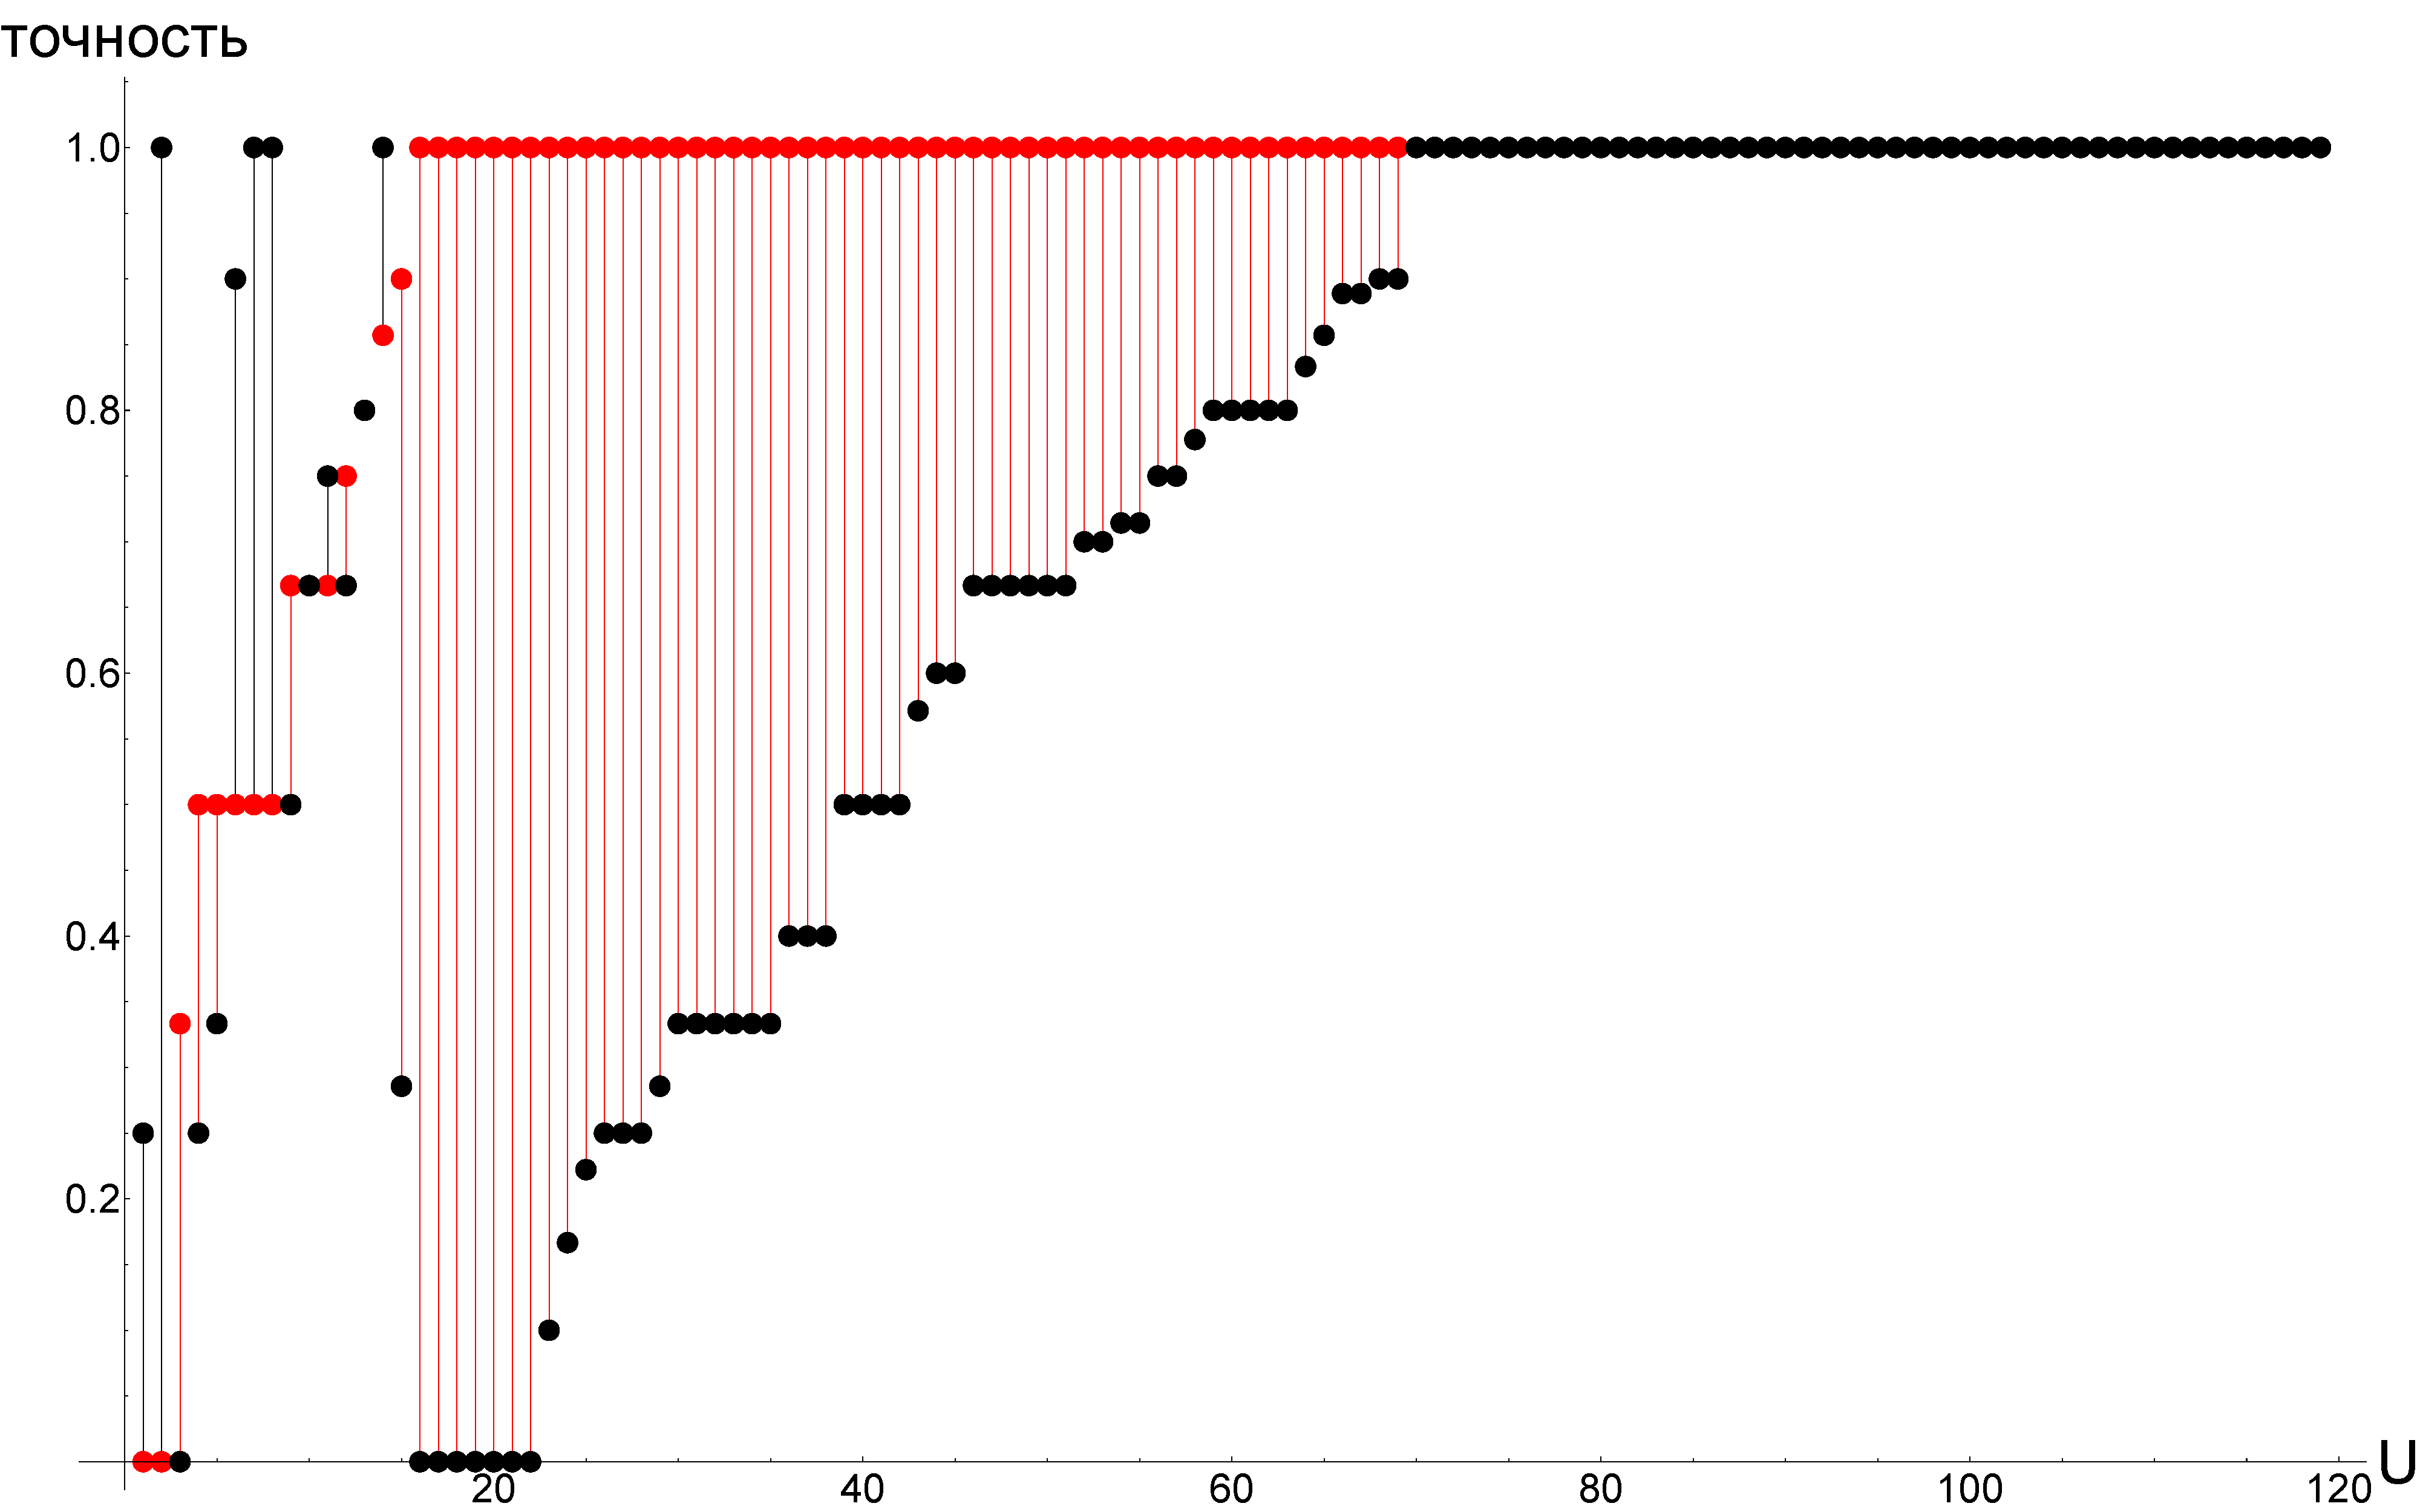
\includegraphics[width=2in,height=1.5in]{pics/transitivity.pdf}
				\end{center}
			\end{figure}
			\begin{center}
				{\bf ---} $\varepsilon_i = 0$\\
				{\color{red} {\bf ---}} $\varepsilon_i = 0,51$.\\
			\end{center}

			\column{.5\textwidth} % Left column and width
			СОМ
			\begin{figure}[h]
				\begin{center}
					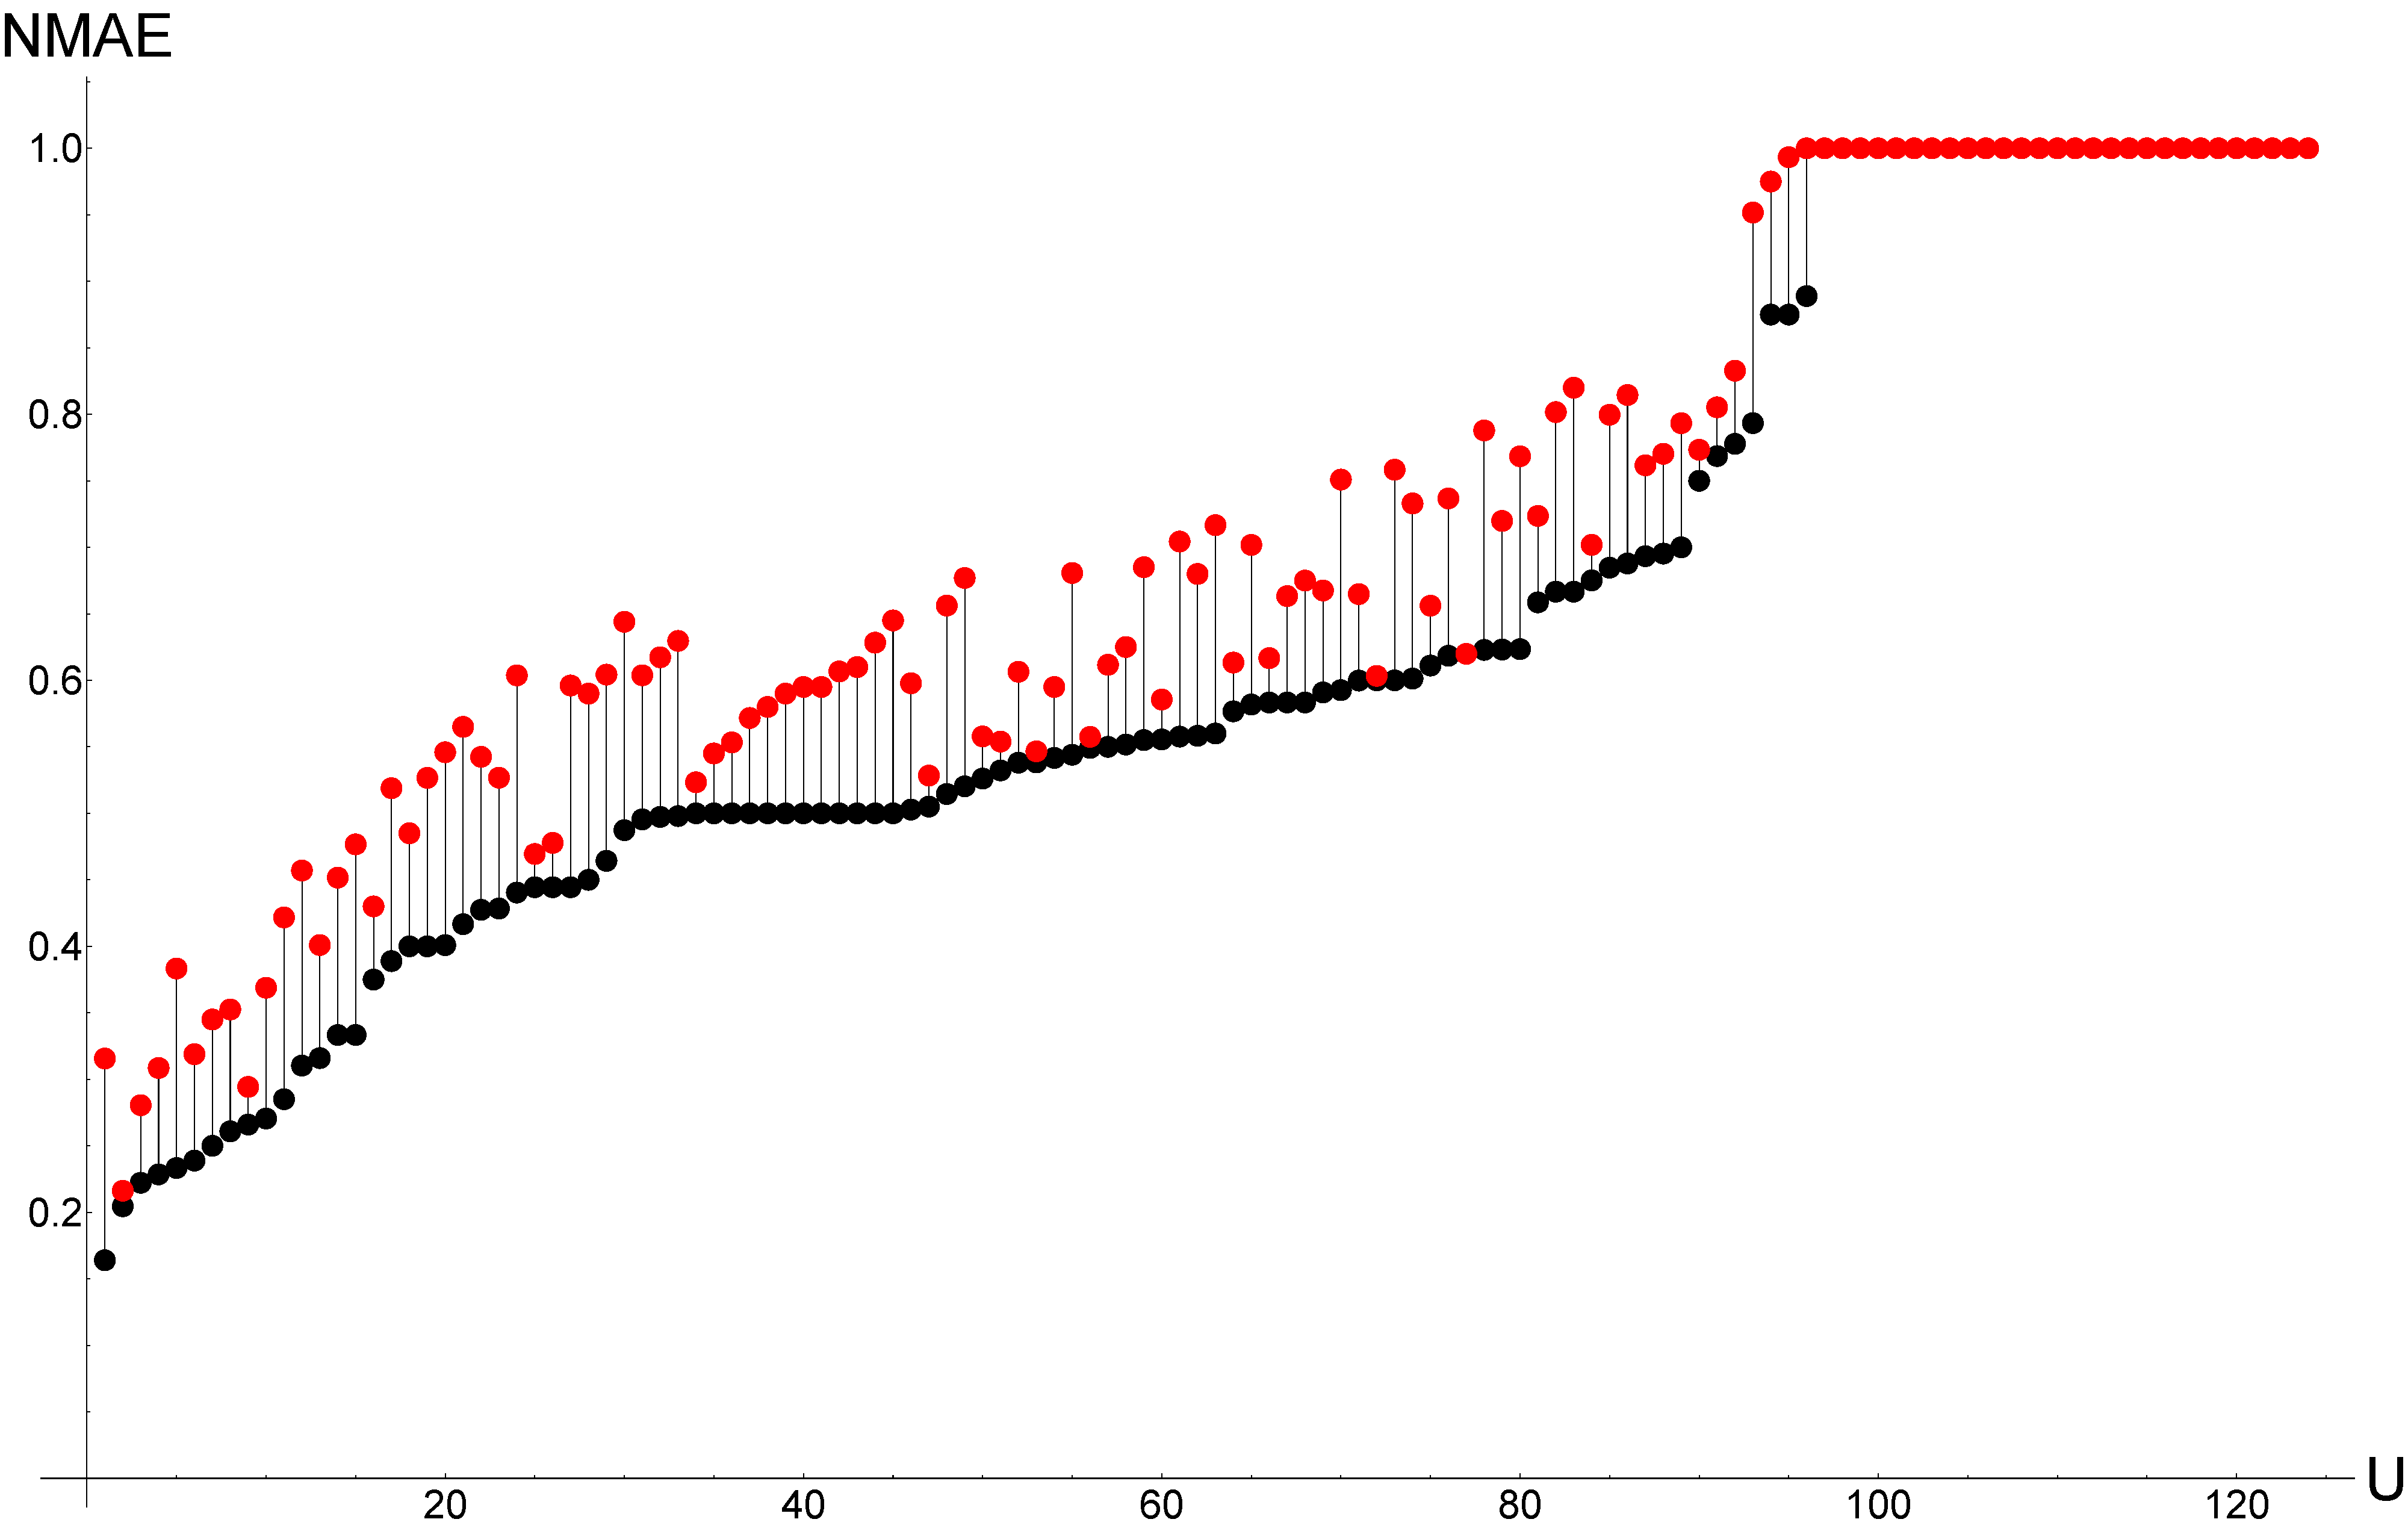
\includegraphics[width=2in,height=1.5in]{pics/ub_transitivity.pdf}
				\end{center}
			\end{figure}
			\begin{center}
				{\bf ---} $\varepsilon_p = 0$\\
				{\color{red} {\bf ---}} $\varepsilon_p = 0,51$\\
			\end{center}
		\end{columns}
	}
\end{frame}


\begin{frame}
	\frametitle{Качество решений задачи $\top$ при применение правила вывода $\Pi_{O}$ в
	нечеткой модели и $OOM$}
	\tiny{
		\begin{columns}[T]
			\column{.7\textwidth} % Left column and width
			\begin{figure}[h]
				\label{pic:topn_hamming}
				\begin{center}
					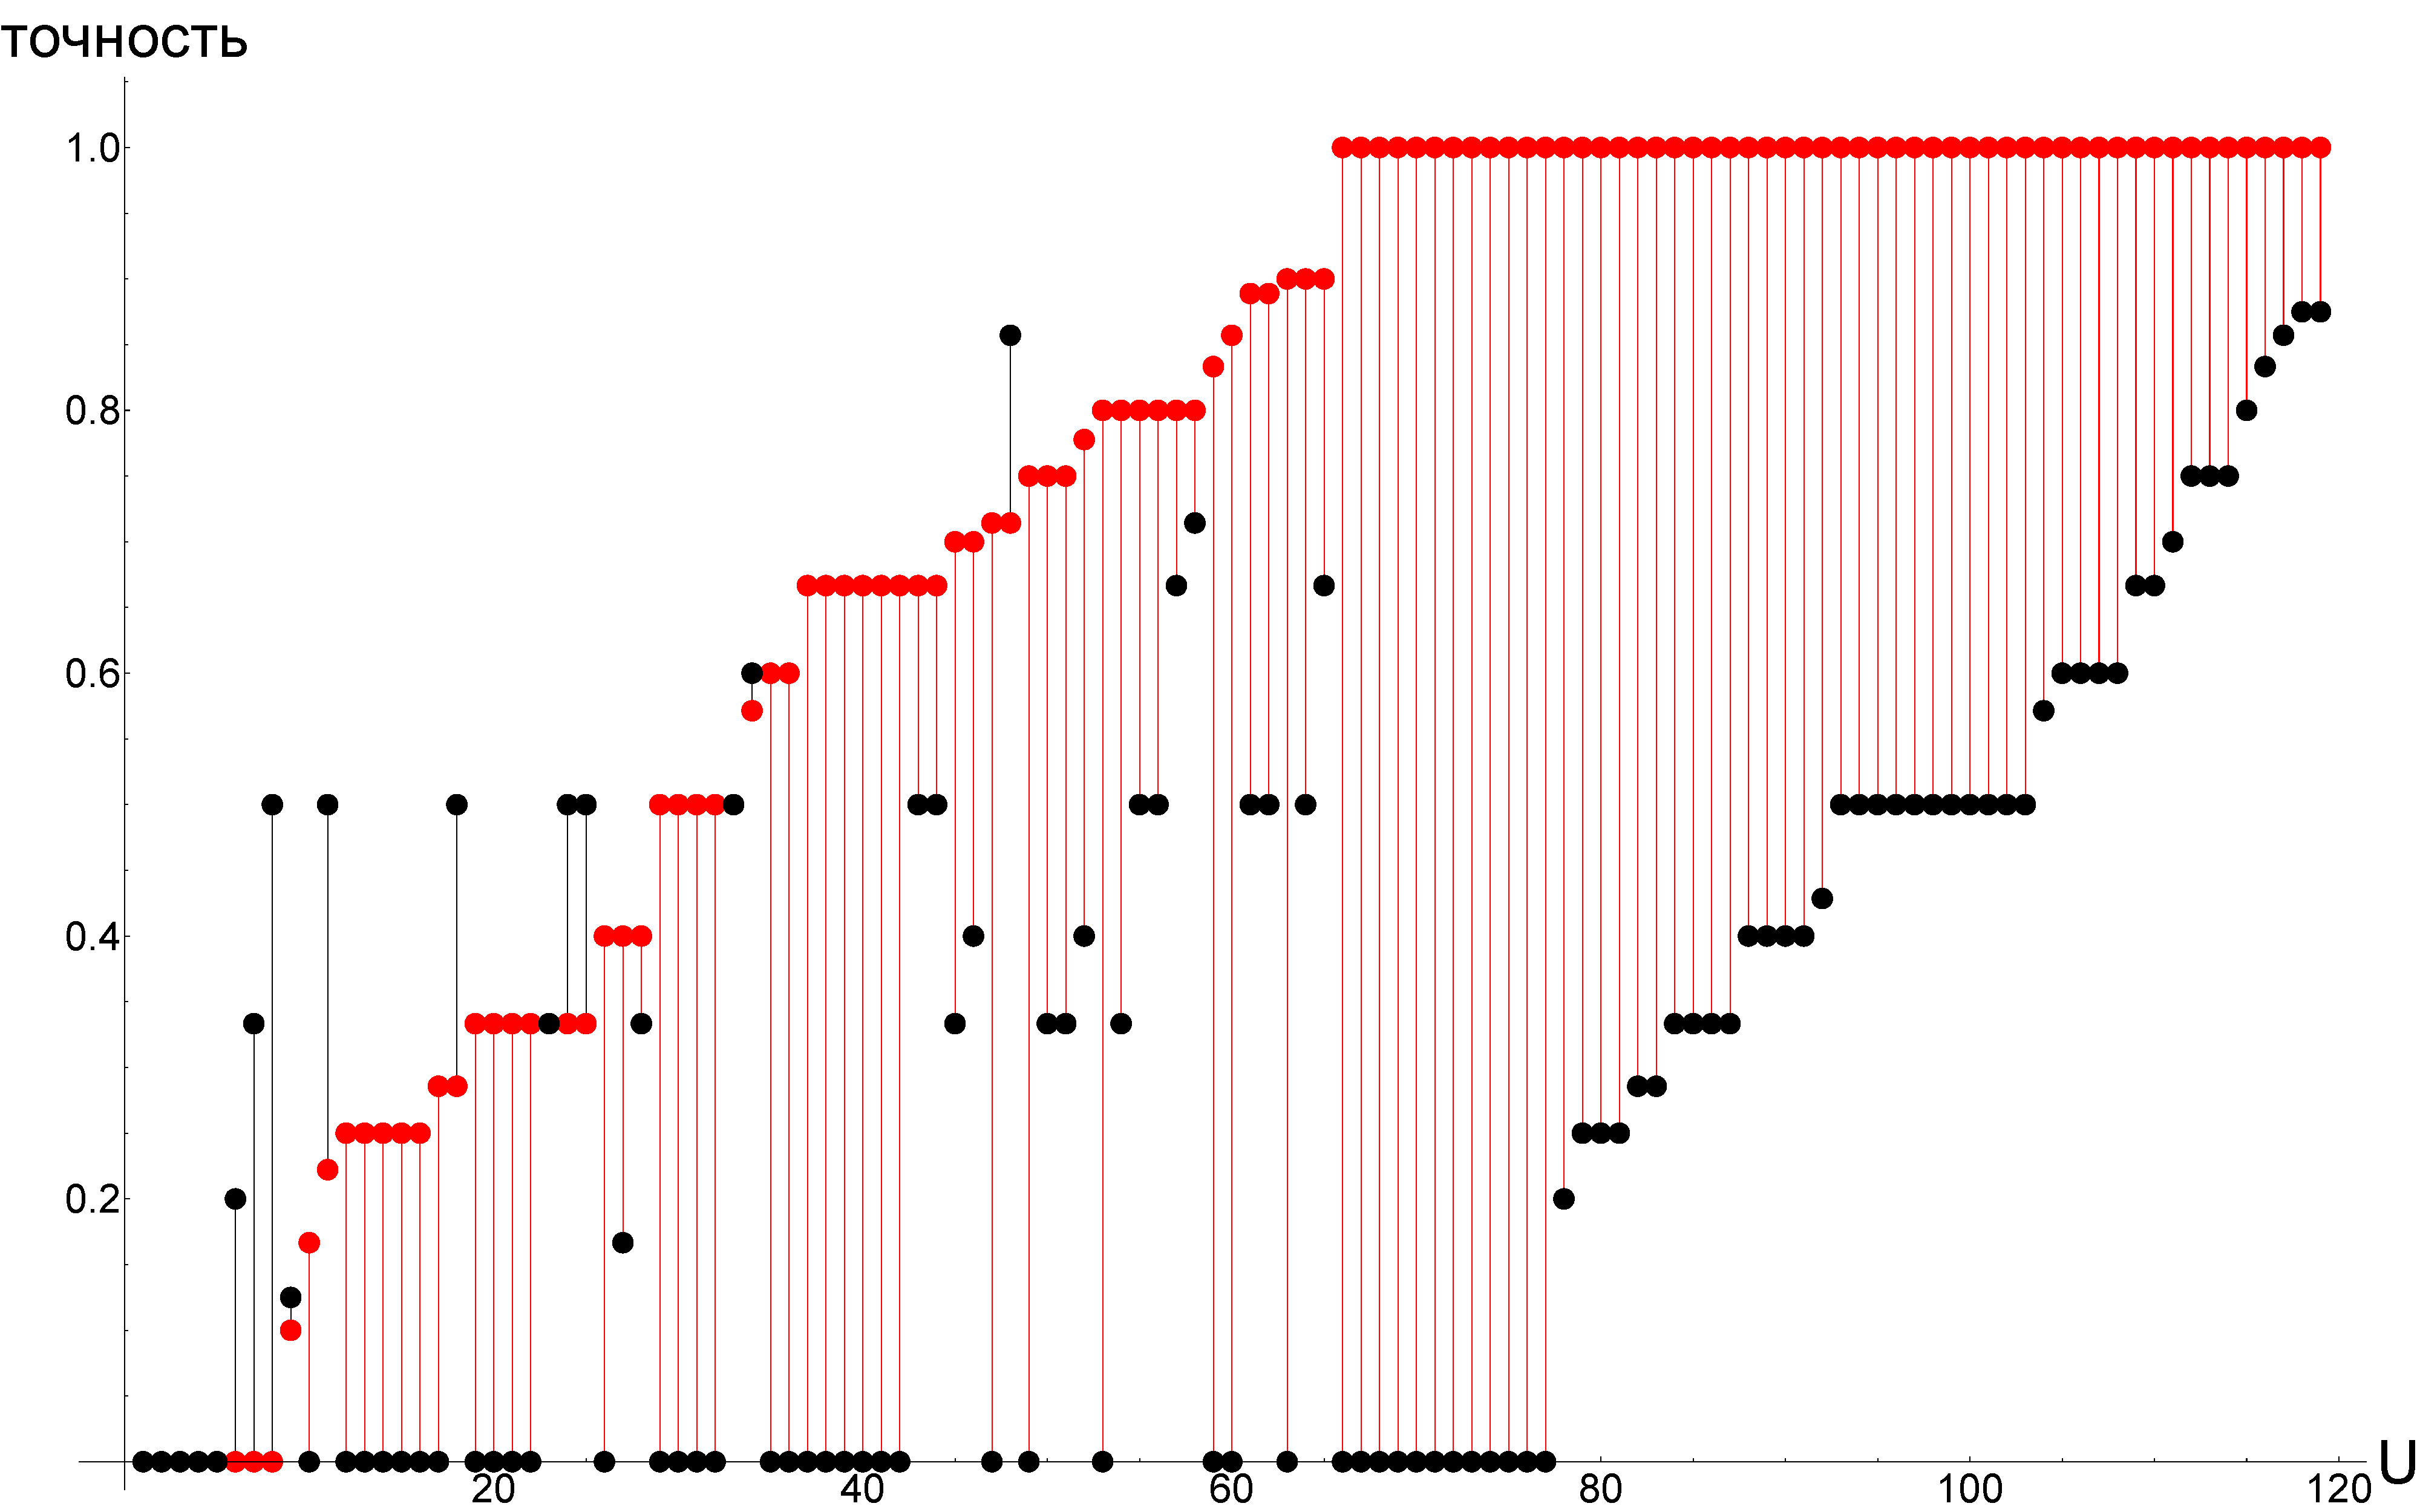
\includegraphics[width=3in,height=2in]{pics/ib_method_in_ib_and_fuzzy_model.pdf}
				\end{center}
			\end{figure}

			\begin{center}
				{\bf ---} $(c_X, c_Y, \Pi_{O})$, $c_X, c_Y$ --- вектора, $\rho_i(i, j) = cos(i, j)$\\
				{\color{red} {\bf ---}} $(c_X, c_Y, \Pi_{O})$, $c_X, c_Y$ --- нечеткие множества, $\rho_i(i, j) = cos(i, j)$
			\end{center}
			%\column{.5\textwidth} % Left column and width
			%\vspace{\baselineskip}
			%\vspace{\baselineskip}
			%\vspace{\baselineskip}
			%\vspace{\baselineskip}
			%\vspace{\baselineskip}
			%\vspace{\baselineskip}
			%\vspace{\baselineskip}
			%\vspace{\baselineskip}

			%\begin{table}[h]
			%	\label{tbl:topn_hamming}
			%	\begin{center}
			%		\begin{tabular}{|c|c|}
			%			\hline
			%			Модель& Точность \\ \hline
			%			ООМ&0,251 \\ \hline
			%			Нечеткая&0,644 \\ \hline
			%		\end{tabular}
			%	\end{center}
			%\end{table}
		\end{columns}
	}
\end{frame}



\begin{frame}
	\frametitle{Качество решений задачи $topN$ при применение $\Pi_O$ в ООМ и $\Pi_{f}$ в
	нечеткой модели}
	\tiny{
		\begin{columns}[T]
			\column{.7\textwidth} % Left column and width
			\begin{figure}[h]
				\begin{center}
					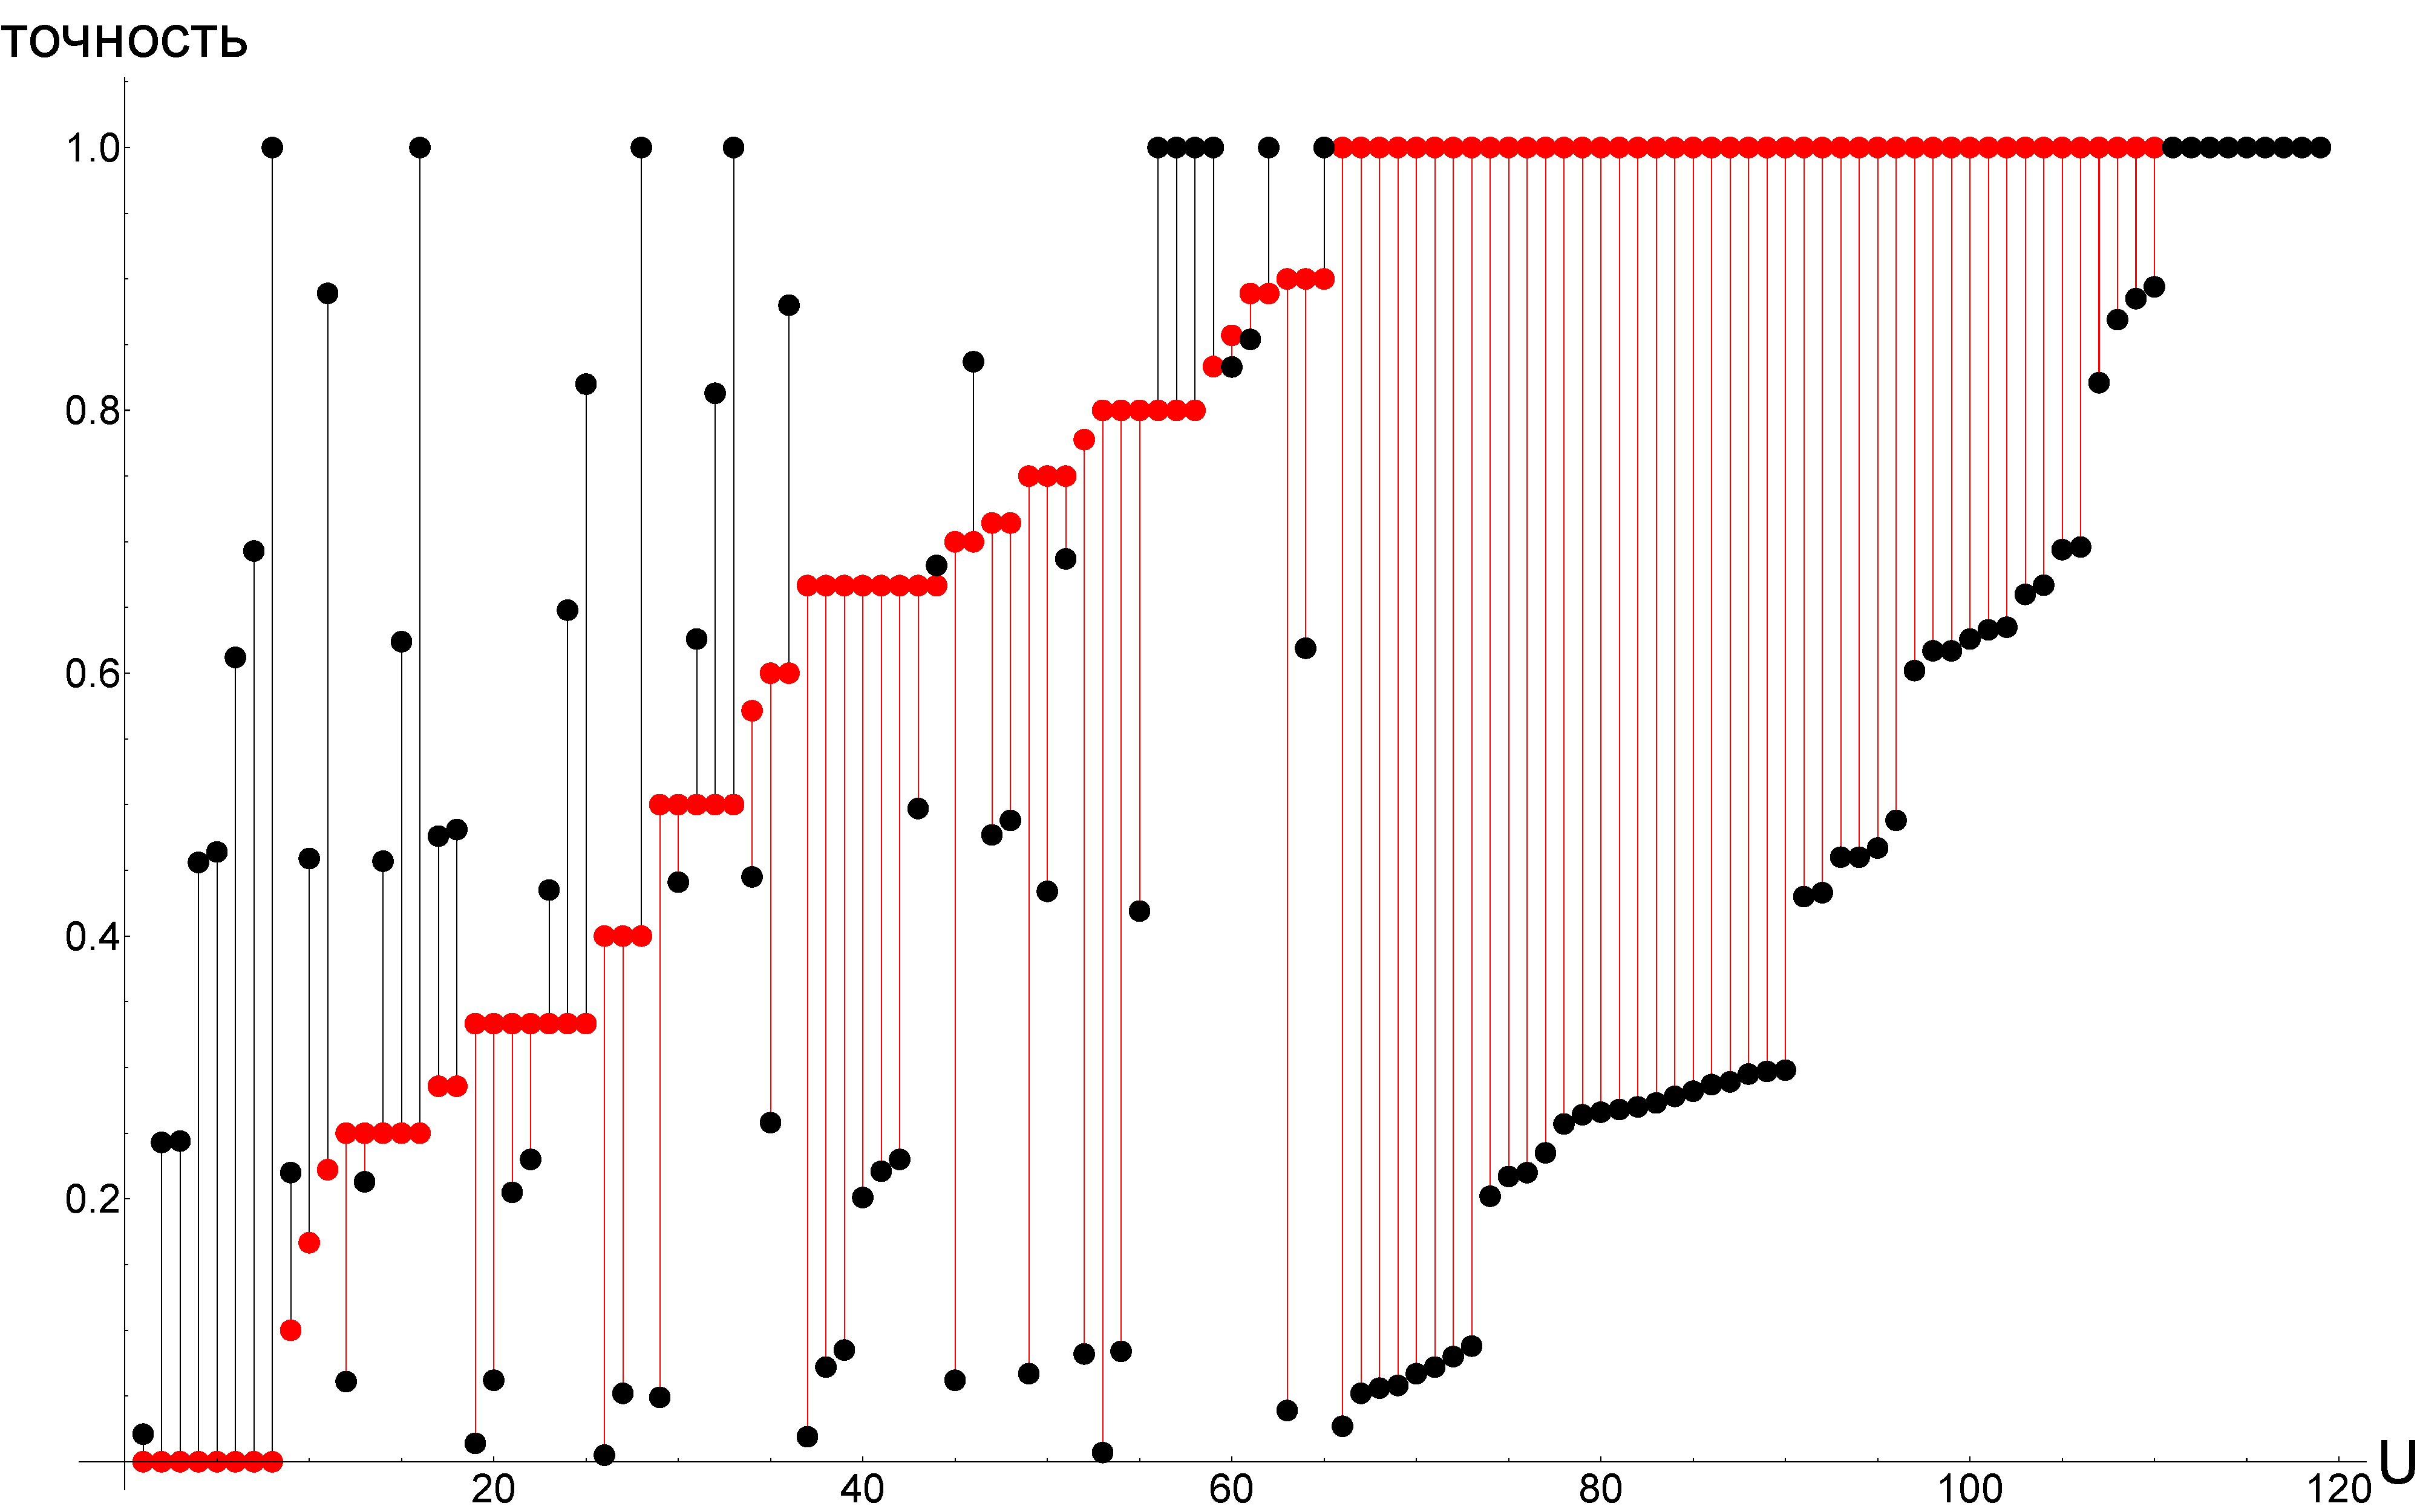
\includegraphics[width=3in,height=2in]{pics/topn_oom_fuzz.pdf}
				\end{center}
			\end{figure}

			%\column{.5\textwidth} % Left column and width
			%\vspace{\baselineskip}
			%\vspace{\baselineskip}
			%\vspace{\baselineskip}
			%\vspace{\baselineskip}
			%\vspace{\baselineskip}
			%\vspace{\baselineskip}
			%\vspace{\baselineskip}
			%\vspace{\baselineskip}

			%\begin{table}[h]
			%	\begin{center}
			%		\begin{tabular}{|c|c|}
			%			\hline
			%			Модель& Точность \\ \hline
			%			ООМ&0,251 \\ \hline
			%			Нечеткая&0,633 \\ \hline
			%		\end{tabular}
			%	\end{center}
			%\end{table}
		\end{columns}
			\begin{center}
				{\bf ---} $(c_X, c_Y, \Pi_{O})$, $c_X, c_Y$ --- вектора, $\rho_i(i, j) = cos(i, j)$\\
				{\color{red} {\bf ---}} $(c_X, c_Y, \Pi_{f})$
			\end{center}
	}
\end{frame}


%\begin{frame}
%	\frametitle{Влияние свойства неоднородности}
%	\tiny{
%		\begin{columns}[T]
%			\column{.5\textwidth} % Left column and width
%			ООМ
%			\begin{figure}[h]
%				\begin{center}
%					\includegraphics[width=2in,height=1.5in]{pics/ib_heterogenity.pdf}
%				\end{center}
%			\end{figure}
%
%			\column{.5\textwidth} % Left column and width
%			Нечеткая модель, $\Pi_f$
%			\begin{figure}[h]
%				\begin{center}
%					\includegraphics[width=2in,height=1.5in]{pics/hetero_fuzz.pdf}
%				\end{center}
%			\end{figure}
%
%		\end{columns}
%	\begin{center}
%		{\bf ---} пороговое значение равно 0,9;\\
%		{\color{red} {\bf ---}} пороговое значение равно 0,49;\\
%	\end{center}
%	}
%\end{frame}


\begin{frame}
	\frametitle{Качество решений задачи $pred$ при применение правила
	вывода $\Pi_{C}$ в
	нечеткой модели и $COM$}
	\tiny{
		\begin{columns}[T]
			\column{.7\textwidth} % Left column and width
			\begin{figure}[h]
				\label{pic:topn_hamming}
				\begin{center}
					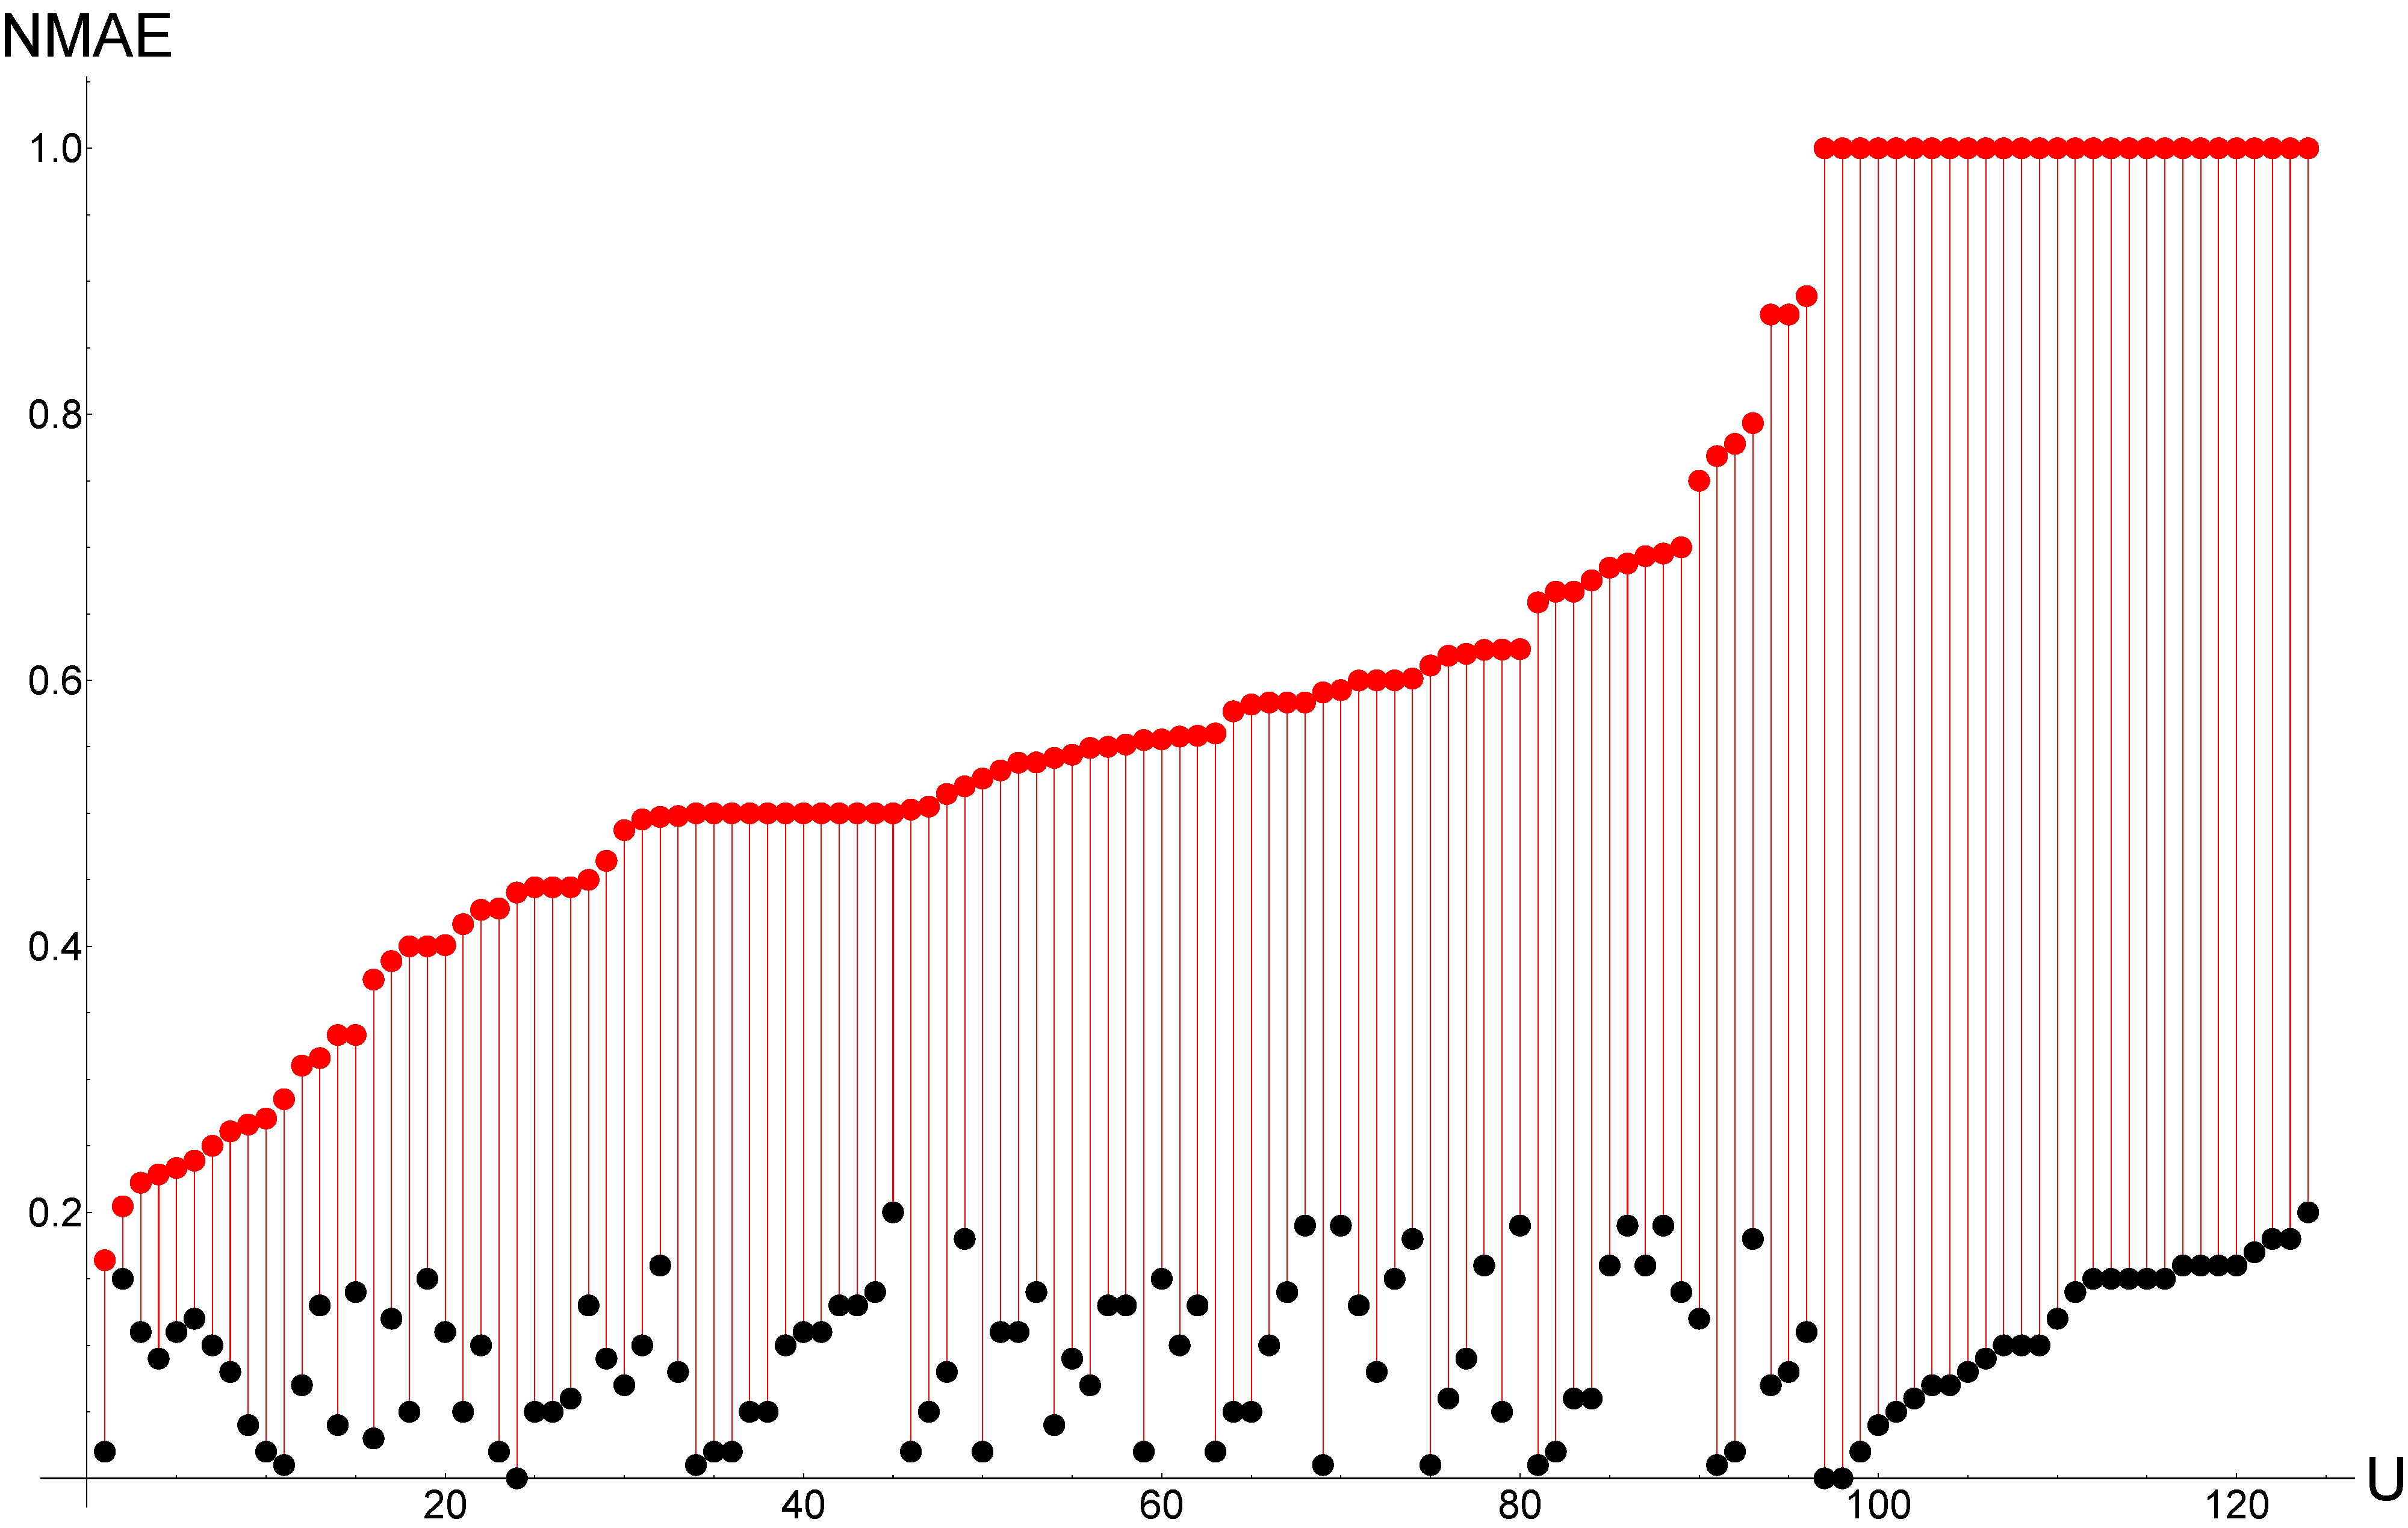
\includegraphics[width=3in,height=2in]{pics/ub_method_in_ub_and_fuzz_model.pdf}
				\end{center}
			\end{figure}

			\begin{center}
				{\bf ---} $(c_X, c_Y, \Pi_{C})$, $c_X, c_Y$ --- выборки, $\rho_u(u,v) = r(u, v)$\\
				{\color{red} {\bf ---}} $(c_X, c_Y, \Pi_{C})$, $c_X, c_Y$ --- нечеткие множества, $\rho_u(u, v) = r(u, v)$
			\end{center}
			%\column{.5\textwidth} % Left column and width
			%\vspace{\baselineskip}
			%\vspace{\baselineskip}
			%\vspace{\baselineskip}
			%\vspace{\baselineskip}
			%\vspace{\baselineskip}
			%\vspace{\baselineskip}
			%\vspace{\baselineskip}
			%\vspace{\baselineskip}

			%\begin{table}[h]
			%	\label{tbl:topn_hamming}
			%	\begin{center}
			%		\begin{tabular}{|c|c|}
			%			\hline
			%			Модель& Точность \\ \hline
			%			СОМ&0,495 \\ \hline
			%			Нечеткая&0,001 \\ \hline
			%		\end{tabular}
			%	\end{center}
			%\end{table}
		\end{columns}
	}
\end{frame}


\begin{frame}
	\frametitle{Качество решений задачи $pred$ при применение $\Pi_C$
	в $COM$ и $\Pi_{f}$ в
	нечеткой модели}
	\tiny{
		\begin{columns}[T]
			\column{.7\textwidth} % Left column and width
			\begin{figure}[h]
				\begin{center}
					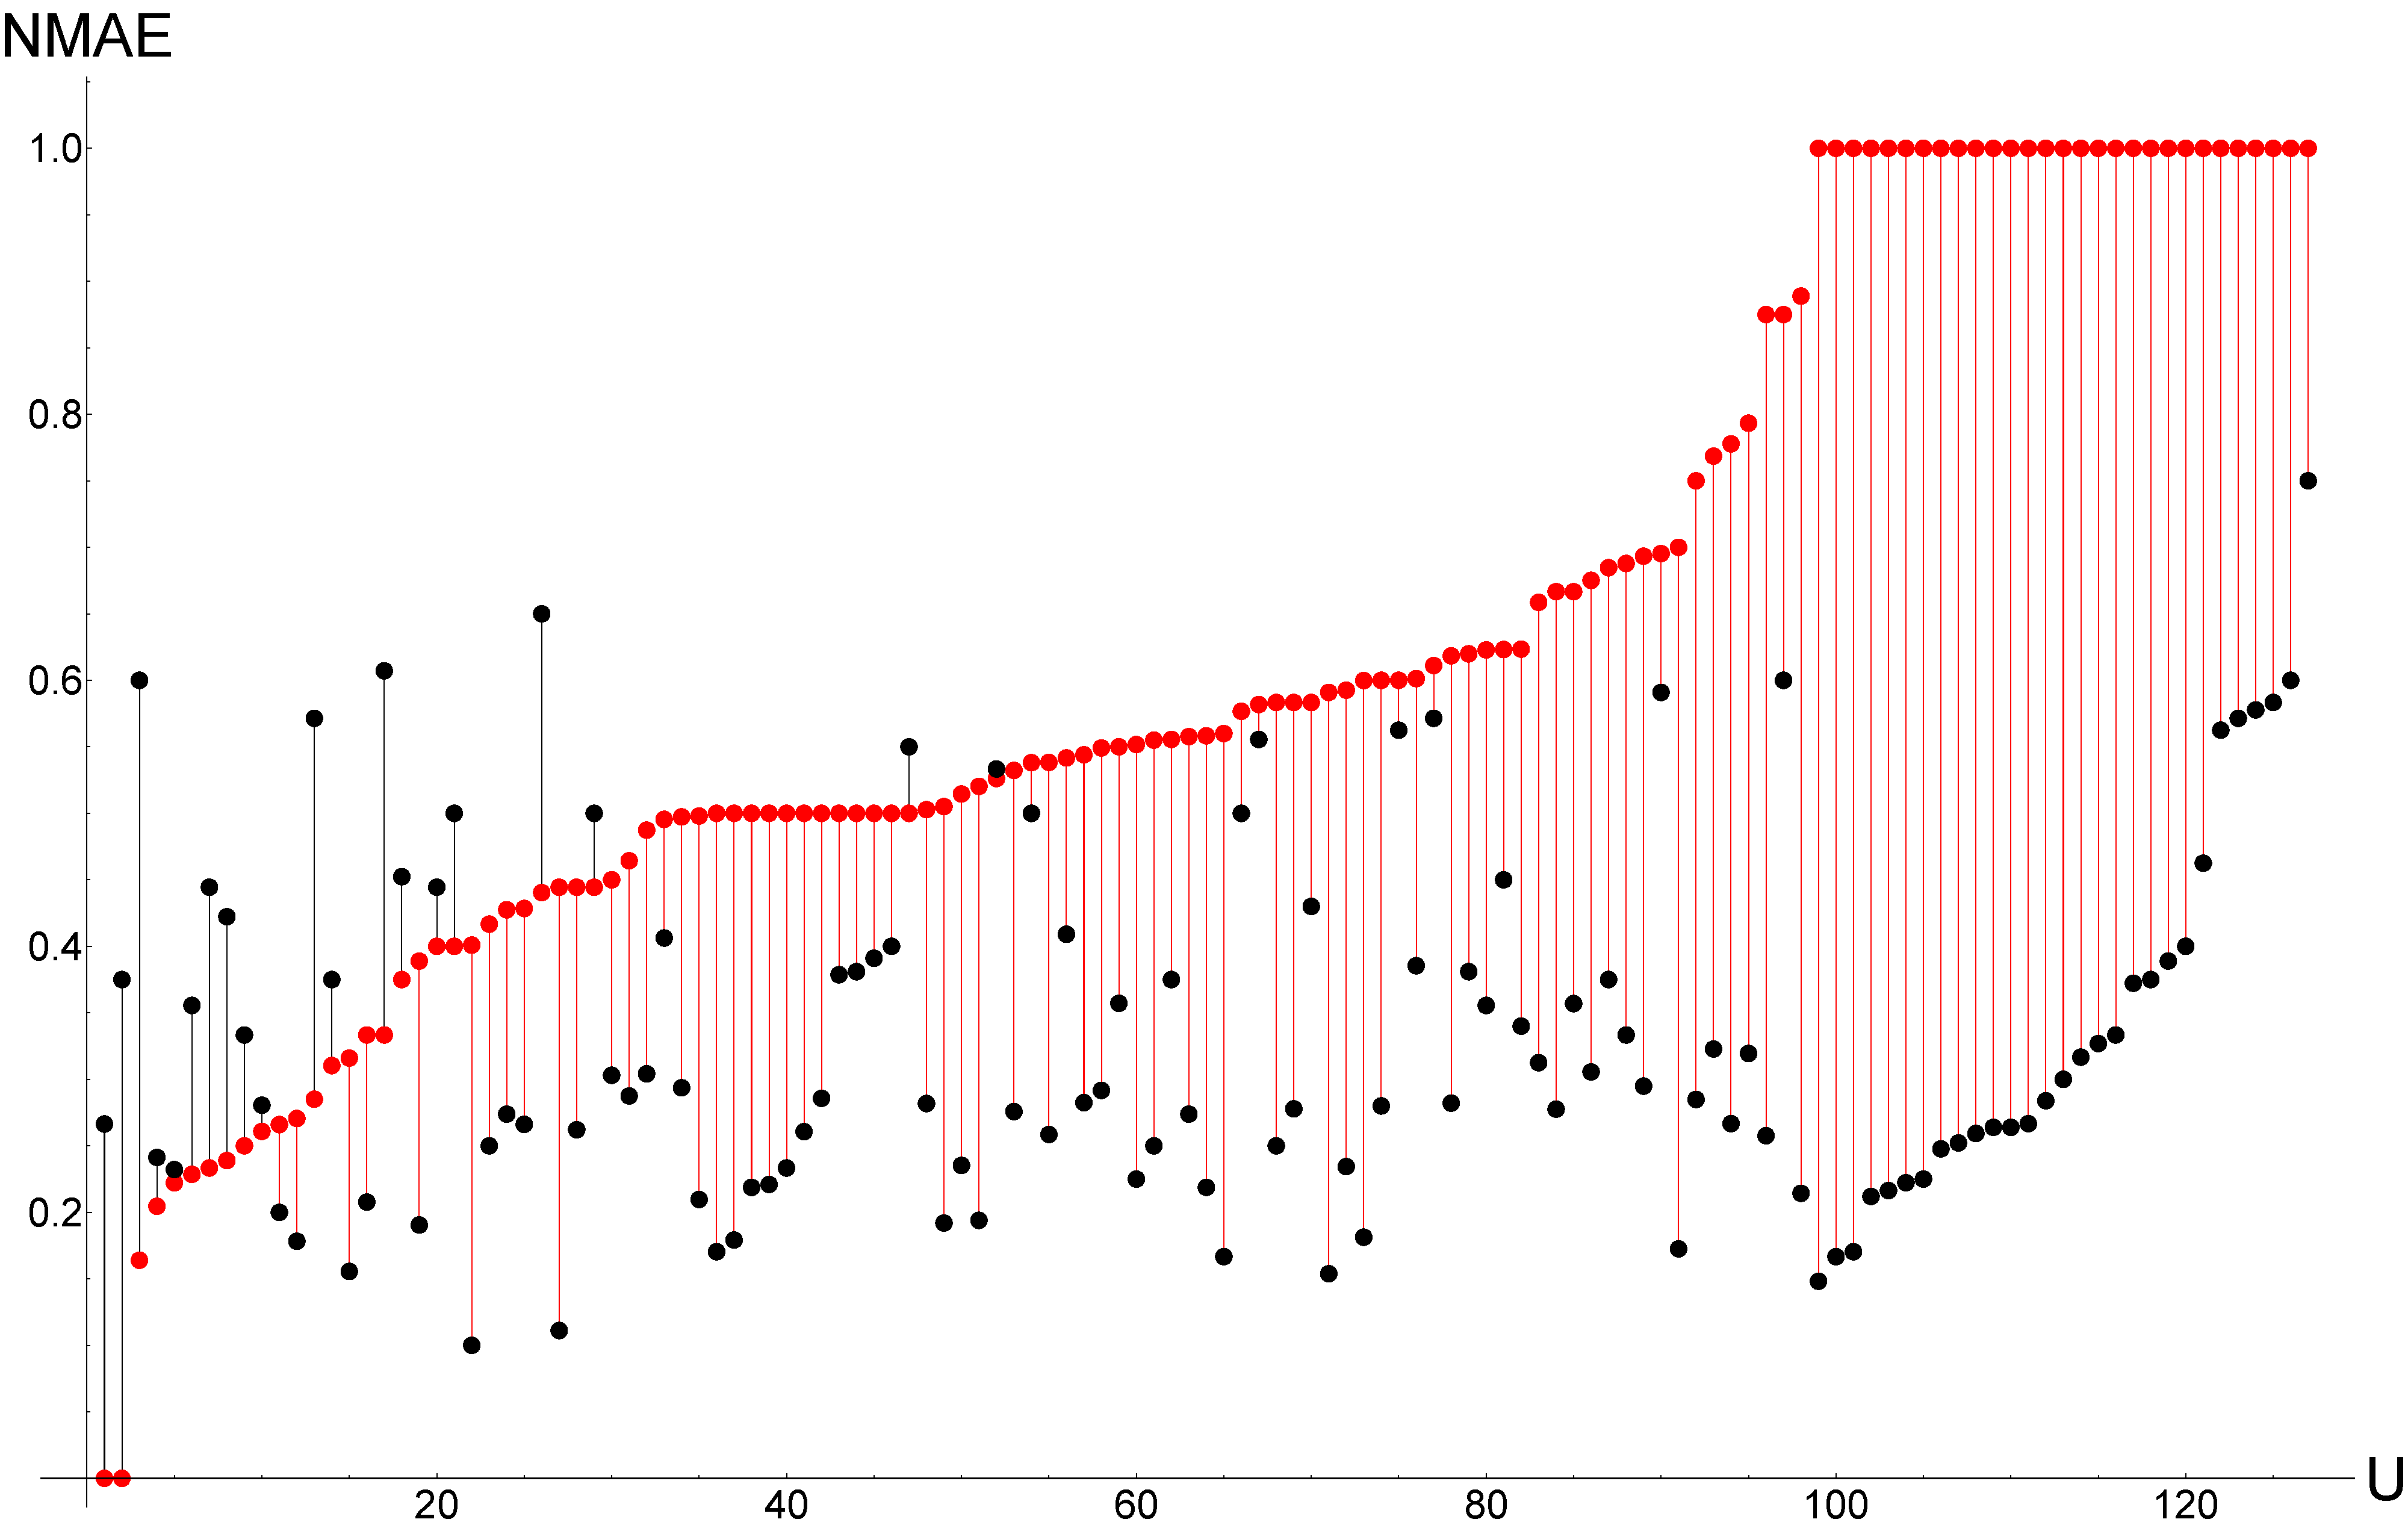
\includegraphics[width=3in,height=2in]{pics/ub_vs_fuzzy.pdf}
				\end{center}
			\end{figure}

			%\column{.5\textwidth} % Left column and width
			%\vspace{\baselineskip}
			%\vspace{\baselineskip}
			%\vspace{\baselineskip}
			%\vspace{\baselineskip}
			%\vspace{\baselineskip}
			%\vspace{\baselineskip}
			%\vspace{\baselineskip}
			%\vspace{\baselineskip}

			%\begin{table}[h]
			%	\begin{center}
			%		\begin{tabular}{|c|c|}
			%			\hline
			%			Модель& Точность \\ \hline
			%			СОМ&0,495\\ \hline
			%			Нечеткая&0,334 \\ \hline
			%		\end{tabular}
			%	\end{center}
			%\end{table}
		\end{columns}
				{\bf ---} $(c_X, c_Y, \Pi_{C})$, $c_X, c_Y$ --- выборки, $\rho_u(u,v) = r(u, v)$\\
				{\color{red} {\bf ---}} $(c_X, c_Y, \Pi_{f})$
	}
\end{frame}


% \begin{frame}
% 	\frametitle{Влияние свойства динамики}
% 	\tiny{
% 		\begin{columns}[T]
% 			\column{.5\textwidth} % Left column and width
% 			ООМ
% 			\begin{figure}[h]
% 				\begin{center}
% 					\includegraphics[width=2in,height=1.5in]{pics/ub_dynamic.pdf}
% 				\end{center}
% 			\end{figure}
% 
% 			\column{.5\textwidth} % Left column and width
% 			Нечеткая модель, $\Pi_f$
% 			\begin{figure}[h]
% 				\begin{center}
% 					\includegraphics[width=2in,height=1.5in]{pics/fuzz_dynamic.pdf}
% 				\end{center}
% 			\end{figure}
% 
% 		\end{columns}
% 	\begin{center}
% 		{\bf ---} пороговое значение равно 0,9;\\
% 		{\color{red} {\bf ---}} пороговое значение равно 0,49;\\
% 	\end{center}
% 	}
% \end{frame}


\begin{frame}
	\frametitle{ПРАКТИЧЕСКАЯ ЦЕННОСТЬ РАБОТЫ}
Основные положения, выводы и рекомендации диссертации ориентированы на широкое применение
разработанных моделей, методики и алгоритмов для реализации рекомендательных систем.
Проведенные исследования и полученные результаты составляют теоретическую основу моделирования
и построения программных комплексов рекомендательных систем.

\begin{center}
	\underline{Самостоятельное практическое значение имеют}
\end{center}
	\begin{enumerate}
		\item Формализованная математическая модель рекомендательной системы;
		\item Алгоритмы решения задч рекомендательных систем;
		\item Программная реализация математической модели рекомендательной системы.
	\end{enumerate}

СВИДЕТЕЛЬСТВА ОБ ОФИЦИАЛЬНОЙ РЕГИСТРАЦИИ ПРОГРАММЫ ДЛЯ ЭВМ № 2013612828 зарегистрированных в РОСПАТЕНТ.

\end{frame}

\begin{frame}
	\frametitle{АПРОБАЦИЯ РАБОТЫ}
	Основные положения диссертации докладывались и обсуждались на конференциях:
	\tiny{
		\begin{enumerate}
			\item XII международная конференция <<Russian Conference on \\Digital Libraries>>
				(г. Казань, 2010 г.);
			\item Молодежная школа-семинар <<Модели и методы исследования систем
				структуры>>, (пос. Дивноморское, 2011, 2014);
			\item Международная конференция <<Управление и оптимизация неголономных
				систем>>,(г. Переславль-Залесский, 2013);
			\item Ученый совет кафедры прикладной математики и информатики
				НИУ ВШЭ (г. Нижний Новгород, 2016);
			\item Ученый совет Исследовательского центра искусственного интеллекта
				ИПС им. А. К. Айламазяна РАН (г. Переславль-Залесский , 2016);
			\item Семинар компании IT-Aces (г. Переславль-Залесский, 2016);
			\item XIX международная конференция <<Data Analytics and Management in Data
				Intensive Domains>> (г. Москва, 2017)
		\end{enumerate}
	}
	\scriptsize{
	\begin{center}
		По результатам исследований опубликовано 8 работ, из них 5 из перечня ВАК.
	\end{center}
	}
\end{frame}

\begin{frame}
	\frametitle{ОСНОВНЫЕ РЕЗУЛЬТАТЫ ДИССЕРТАЦИОННОЙ РАБОТЫ}
	\begin{enumerate}
		\item получены достаточные условия, при выполнении которых
			коллаборативная модель РС гарантирует формирование качественного
			результата решения задач;
		\item определены свойства исходных данных, влияющих на качество
			решения, сформированного при применении коллаборативной модели;
		\item разработана модель РС, основанная на теории нечетких множеств.
			Разработанная модель является эффективной модификацией
			коллаборативной модели;
		\item разработано программное обеспечение, с помощью которого было
			проведено тестирование разработанной и коллаборативной моделей.
			Получены практические результаты, которые
			подтверждют теоретические выводы о том, что разработанная модель
			является эффективной модификацией коллаборативной.
	\end{enumerate}
\end{frame}

% \begin{frame}
% 	\frametitle{Свидетельство о регистрации программного обеспечения}
% 	\tiny{
% 		\begin{figure}[h]
% 			\begin{center}
% 				\includegraphics[width=2in,height=3in]{pics/svidetelstvo.pdf}
% 			\end{center}
% 		\end{figure}
% 	}
% \end{frame}

%\begin{frame}
%	\frametitle{Опубликованные статьи. Рецензируемые журналы.}
%	\tiny{
%		\begin{enumerate}
%			\item Понизовкин Д. М.
%				Оптимальное распределение проектов при проведении экспертизы / Д. М. Понизовкин, С. А. Амелькин //
%				Электронные библиотеки: Перспективные Методы и Технологии,
%				Электронные коллекции. --- 2010. --- С. 524-525.
%				% электронный
%			\item Амелькин С. А, Д. М. Понизовкин. Оптимальное проведение экспертизы образовательных процессов / С. А. Амелькин, Д. М. Понизовкин //
%				Труды XVII Всероссийской научно-методической конференции Телематика’2010,
%				Санкт-Петербург: Университетские телекоммуникации. --- 2010. ---
%				№ 1, С. 158-159.
%		\end{enumerate}
%	}
%\end{frame}

\begin{frame}
МАТЕМАТИЧЕСКАЯ МОДЕЛЬ РЕКОМЕНДАТЕЛЬНОЙ\\
\hspace{12mm}СИСТЕМЫ НА НЕЧЕТКИХ МНОЖЕСТВАХ\\
\hspace{18mm}КАК ЭФФЕКТИВНАЯ МОДИФИКАЦИЯ\\
\hspace{22mm}КОЛЛАБОРАТИВНОЙ МОДЕЛИ

\hfill \break
\begin{center}
Диссертация на соискание степени кандидата технических наук
\end{center}
\hfill \break
Специальность: 05.13.18 --- Математическое моделирование,\\
\hspace{25mm} численные методы и комплексы программ\\
\hfill \break
	\begin{center}
Научный руководитель: к.т.н., С.А. Амелькин
	\end{center}
	\begin{center}
Соискатель: Д.М. Понизовкин
	\end{center}
\end{frame}

%%%%%%% END
\end{document}
